% ============================================================
%  Astera Labs 全面调研报告
%  编译引擎：XeLaTeX
%  文档类：ctexart (中文文章)
%  日期：2026-05-19
%
%  编译命令：xelatex asteralabs_report.tex
%  编译两次以确保交叉引用正确
% ============================================================

\documentclass[11pt,a4paper]{ctexart}

% ---- 页面设置 ----
\usepackage{geometry}
\geometry{margin=2.5cm}

% ---- 中文支持 ----
\setCJKmainfont{Songti SC}
\setCJKsansfont{Heiti SC}
\setCJKmonofont{STFangsong}

% ---- 图形与绘图 ----
\usepackage{graphicx}
\usepackage{tikz}
\usetikzlibrary{positioning, calc, shapes.geometric, arrows.meta, backgrounds, fit, chains}
\usepackage{caption}
\usepackage{subcaption}
\graphicspath{{./figures/}}

% ---- 表格 ----
\usepackage{booktabs}
\usepackage{tabularx}
\usepackage{multirow}
\usepackage{array}
\usepackage[table]{xcolor}

% ---- 数学 ----
\usepackage{amsmath,amssymb}
\usepackage{mathtools}

% ---- 代码 ----
\usepackage{listings}
\lstset{
    basicstyle=\ttfamily\small,
    keywordstyle=\color{blue}\bfseries,
    commentstyle=\color{darkgreen},
    stringstyle=\color{darkred},
    numbers=left,
    numberstyle=\tiny\color{gray},
    backgroundcolor=\color{mygray},
    breaklines=true,
    frame=single,
    tabsize=2
}

% ---- 链接与引用 ----
\usepackage{hyperref}
\hypersetup{
    colorlinks=true,
    linkcolor=darkblue,
    urlcolor=darkblue,
    citecolor=darkblue
}

% ---- 其他工具 ----
\usepackage{enumitem}
\usepackage{fancyhdr}
\usepackage{changelog}
\usepackage{xurl}  % 支持长URL换行
\usepackage{twemojis}
\usepackage{tcolorbox}
\tcbuselibrary{skins}

% ---- 自定义颜色 ----
\definecolor{darkgreen}{RGB}{0,128,0}
\definecolor{darkred}{RGB}{180,0,0}
\definecolor{darkblue}{RGB}{0,0,139}
\definecolor{gold}{RGB}{200,150,0}
\definecolor{mygray}{RGB}{245,245,245}
\definecolor{t1green}{RGB}{220,255,220}
\definecolor{t2blue}{RGB}{200,220,255}
\definecolor{t3yellow}{RGB}{255,255,200}
\definecolor{t4orange}{RGB}{255,230,200}
\definecolor{t5red}{RGB}{255,200,200}

% ---- 自定义命令 ----
\newcommand{\sourceT}[1]{{\small\textcolor{darkblue}{[T#1]}}}
\newcommand{\unverified}{{\textcolor{darkred}{\textbf{[未确认]}}}}
\newcommand{\speculation}{{\textcolor{orange}{\textbf{[推测]}}}}
\newcommand{\marketing}{{\textcolor{orange}{\textbf{[可能为营销语言]}}}}
\newtcolorbox{warningblock}{
    colback=red!5!white,
    colframe=red!75!black,
    fonttitle=\bfseries,
    title={\twemoji{warning} 注意},
    sharp corners,
    boxrule=0.8pt
}
% ---- 文档信息 ----
\title{\textbf{Astera Labs 全面调研报告}\\[0.3cm]
       \large 工程级别、产业级别的深度分析}
\author{葛良晨}
\date{\today}

\begin{document}

\maketitle

\begin{abstract}
\noindent 本报告对 Astera Labs（Nasdaq: ALAB）进行了工程级别、产业级别的全面调研。
覆盖公司定位与历史、全产品线（Scorpio/Aries/Leo/Taurus/COSMOS）、
核心技术与架构、竞争格局、CXL/PCIe/Retimer技术深度、财务分析、
以及最终投资与产业评估。

\textbf{核心发现}：Astera Labs 是全球唯一横跨 PCIe Retimer + PCIe Switch + CXL Controller + Ethernet Cable + 软件管理平台的连接芯片公司。
其 Scorpio X-Series（320-lane memory semantic fabric switch）是目前唯一基于 PCIe 的 AI 优化大 radix fabric switch，
在 hyperscaler GPU 集群中具有独特定位。FY2025 收入 \$852.5M，毛利率 75-76\%，已实现正盈利。
主要风险包括客户集中度、Broadcom 竞争威胁与 AI CAPEX 周期依赖。

\textbf{研究方法}：所有关键结论均标注信息来源等级 [T1]（官方可验证文档）至 [T5]（社区推测）。
无法确认的信息明确标注``\unverified{}''或``\speculation{}''。
报告中的技术架构图均为 TikZ 原创绘制。

\textbf{声明}：本报告不构成投资建议。所有分析基于公开信息。
\end{abstract}

\tableofcontents
\clearpage

% ============================================================
%  PART 1: 公司整体定位
% ============================================================
% ============================================================
%  Part 1: 公司整体定位
% ============================================================

\section{公司整体定位}

\subsection{公司基本信息}

Astera Labs, Inc.（纳斯达克代码：ALAB）是一家专注于 AI 基础设施连接方案的 fabless 半导体公司。
以下为公司核心信息：

\begin{table}[htb]
    \centering
    \caption{Astera Labs 公司概览}
    \label{tab:company-overview}
    \begin{tabular}{lll}
        \toprule
        \textbf{属性} & \textbf{内容} & \textbf{来源} \\
        \midrule
        公司全称 & Astera Labs, Inc. & \sourceT{1} SEC \\
        成立时间 & 2017 年 & \sourceT{2} Wikipedia \\
        总部 & Santa Clara, CA → 2025 年迁至 San Jose & \sourceT{2} Wikipedia \\
        上市时间 & 2024 年 3 月 (Nasdaq: ALAB) & \sourceT{1} SEC \\
        IPO 估值 & $\sim$\$5.5B, 募资 $\sim$\$713M & \sourceT{2} Wikipedia \\
        商业模式 & Fabless (无晶圆厂设计公司) & \sourceT{2} 官方 \\
        晶圆代工 & TSMC & \sourceT{3} SemiAnalysis \\
        行业分类 & SIC 3674 (Semiconductors \& Related Devices) & \sourceT{1} SEC \\
        员工规模 & 未公开精确数字 & \unverified{} \\
        \bottomrule
    \end{tabular}
\end{table}

\subsection{创始团队}

三位创始人全部来自 Texas Instruments（TI）：
\begin{itemize}
    \item \textbf{Jitendra Mohan} — CEO
    \item \textbf{Sanjay Gajendra}
    \item \textbf{Casey Morrison}
\end{itemize}

三人在 TI 共事后，观察到数据中心连接技术无法跟上 AI/ML 的发展步伐，
在 Sanjay Gajendra 的车库中开始创业。TI 背景意味着创始团队在模拟/混合信号设计领域有深厚积累——
这正是高速 SerDes/Retimer 产品的核心能力需求。\sourceT{2}

\subsection{融资与 IPO 历史}

\begin{table}[htb]
    \centering
    \caption{融资历史}
    \label{tab:funding}
    \begin{tabular}{llll}
        \toprule
        \textbf{轮次} & \textbf{时间} & \textbf{金额} & \textbf{关键投资者} \\
        \midrule
        Series B & 2020 年 4 月 & 未公开 & Avigdor Willenz, Intel Capital, Ron Jankov, Sutter Hill Ventures \\
        Series C & 2021 年 9 月 & \$50M & Fidelity Investments 领投，估值 $\sim$\$950M \\
        Series D & 2022 年 11 月 & \$150M & 估值超过 \$3B \\
        IPO & 2024 年 3 月 & \$713M & Morgan Stanley, JPMorgan 承销，估值 $\sim$\$5.5B \\
        \bottomrule
    \end{tabular}
\end{table}

\textbf{重要事件}：在 IPO 之前，Astera Labs 曾拒绝 Marvell 的收购要约。\sourceT{3}
Intel Capital 作为早期投资方值得注意——Intel 是 PCIe 和 CXL 标准的主要推动者之一，
这个关系可能为 Astera Labs 的产品路线图提供了标准层面的前瞻性指导。

\textbf{Post-IPO 扩展}：
\begin{itemize}
    \item 2024 年：扩展台湾业务，加强本地服务器 ODM 合作
    \item 2024 年底：在印度班加罗尔设立研发中心
    \item 2025 年 6 月：总部迁至 San Jose 新园区，面积扩大三倍
    \item 2025 年底：加入 Arm Total Design 生态系统
    \item 2026 年 2 月：宣布在特拉维夫设立新的设计中心
\end{itemize}
\sourceT{2}

\subsection{公司核心定位}

Astera Labs 的核心定位可用三个层次描述：

\begin{enumerate}
    \item \textbf{物理层}：通过 Aries Retimer/Cable Module 解决高速信号传输问题
    \item \textbf{架构层}：通过 Scorpio Fabric Switch 解决 GPU/NIC/Storage 之间的交换互连问题
    \item \textbf{系统层}：通过 COSMOS 提供全链路的 telemetry 和 fleet management
\end{enumerate}

这三个层次构成了一个完整的``连接平台''——从铜线到软件管理。公司的核心 slogan 是
\textbf{``Purpose-Built Connectivity for Rack-Scale AI''}。

\begin{figure}[htb]
    \centering
    \begin{tikzpicture}[
        box/.style={rectangle, draw=darkblue, fill=blue!5, thick, minimum width=6cm, minimum height=0.9cm, align=center, rounded corners=5pt},
        arrow/.style={->, >=Stealth, thick}
    ]
        \node[box, fill=darkred!10] (SLOGAN) at (0,0) {\textbf{``Purpose-Built Connectivity for Rack-Scale AI''}};
        \node[box, fill=darkgreen!10, below=0.2cm of SLOGAN] (POS) {定位：AI Infra 连接层供应商};
        \node[box, fill=yellow!10, below=0.2cm of POS] (DIFF) {差异化：Open Standards (PCIe/CXL vs 私有 NVLink)};
    \end{tikzpicture}
    \caption{Astera Labs 核心定位}
    \label{fig:positioning}
\end{figure}

\subsection{产业链位置}

Astera Labs 采用 fabless 模式：芯片设计（内部）→ TSMC 代工 → OSAT 封测 →
供货给 hyperscaler/Server OEM/GPU Vendor。其产业链位置如下图所示：

\begin{figure}[htb]
    \centering
    \begin{tikzpicture}[
        node distance=1.0cm and 0.8cm,
        box/.style={rectangle, draw=darkblue, thick, minimum width=2.5cm, minimum height=0.9cm, align=center, rounded corners=3pt},
        highlight/.style={rectangle, draw=darkred, fill=red!10, thick, minimum width=2.8cm, minimum height=0.9cm, align=center, rounded corners=3pt},
        arrow/.style={->, >=Stealth, thick}
    ]
        \node[box, fill=gray!10] (EDA) {EDA/IP\\Synopsys/Cadence};
        \node[box, fill=gray!10, right=of EDA] (FAB) {晶圆代工\\TSMC};
        \node[box, fill=gray!10, right=of FAB] (OSAT) {封装测试\\OSAT};

        \node[highlight, below=of FAB] (AST) {\textbf{Astera Labs}\\\textbf{Fabless Chip Designer}};

        \node[box, fill=blue!5, below left=of AST] (P1) {Scorpio\\Fabric Switch};
        \node[box, fill=blue!5, below=of AST] (P2) {Aries\\Retimer/Cable};
        \node[box, fill=blue!5, below right=of AST] (P3) {Leo/Taurus\\CXL/Ethernet};

        \node[box, fill=darkgreen!10, below=of P2, minimum width=3.2cm] (CUST) {Hyperscalers\\+ Server OEM\\+ GPU Vendor};

        \draw[arrow] (EDA) -- (AST);
        \draw[arrow] (FAB) -- (AST);
        \draw[arrow] (OSAT) -- (AST);
        \draw[arrow] (AST) -- (P1);
        \draw[arrow] (AST) -- (P2);
        \draw[arrow] (AST) -- (P3);
        \draw[arrow] (P1) -- (CUST);
        \draw[arrow] (P2) -- (CUST);
        \draw[arrow] (P3) -- (CUST);
    \end{tikzpicture}
    \caption{Astera Labs 产业链位置}
    \label{fig:supply-chain}
\end{figure}

\subsection{核心概念解释}

\subsubsection{Rack-Scale AI}

单个 AI 服务器已无法容纳所需 GPU 数量，多个服务器需跨机架（rack）协同工作。
GPT-4 级别模型训练需要数千 GPU 互连，推理大模型也需要多 GPU。
AI 模型规模每 18-24 个月增长约 10$\times$（比摩尔定律更快），
单个 GPU 的 HBM 容量（80GB-192GB）远小于模型所需（GPT-4 约 1.76T 参数需要 $>$3.5TB 内存用于推理）。
因此 GPU 必须互连形成逻辑上的``大 GPU''，连接带宽决定 GPU 利用率。\sourceT{3}

\begin{figure}[htb]
    \centering
    \begin{tikzpicture}[
        scale=0.85,
        rack/.style={rectangle, draw=darkblue, fill=blue!3, thick,
                     minimum width=2.8cm, minimum height=3.8cm, rounded corners=3pt},
        gpu/.style={rectangle, draw=darkred, fill=red!8, thick,
                    minimum width=1.0cm, minimum height=0.6cm, align=center,
                    font=\tiny, rounded corners=1pt},
        nic/.style={rectangle, draw=darkgreen, fill=green!10, thick,
                    minimum width=1.0cm, minimum height=0.5cm, align=center,
                    font=\tiny, rounded corners=1pt},
        scorp/.style={rectangle, draw=gold, fill=yellow!10, thick,
                      minimum width=1.05cm, minimum height=0.55cm, align=center,
                      font=\tiny, rounded corners=2pt},
        connect/.style={-, thick, darkblue!70},
        soArrow/.style={->, >=Stealth, very thick, darkgreen!65},
        racklabel/.style={font=\footnotesize\bfseries, above=0.15cm},
    ]
    % ===== Rack 1: Scale-Up Domain (6 GPUs, 2 cols × 3 rows) =====
    \node[rack] (R1) {};
    \node[racklabel] at (R1.north) {Rack 1 (Scale-Up Domain)};

    \node[gpu] (G1)  at ($(R1.center)+(-0.68, 1.1)$)  {GPU};
    \node[gpu] (G2)  at ($(R1.center)+( 0.68, 1.1)$)  {GPU};
    \node[gpu] (G3)  at ($(R1.center)+(-0.68, 0.35)$) {GPU};
    \node[gpu] (G4)  at ($(R1.center)+( 0.68, 0.35)$) {GPU};
    \node[gpu] (G5)  at ($(R1.center)+(-0.68,-0.4)$)  {GPU};
    \node[gpu] (G6)  at ($(R1.center)+( 0.68,-0.4)$)  {GPU};

    \node[scorp] (S1) at ($(R1.center)+(0, -1.15)$) {Scorpio};
    \node[nic, right=0.25cm of S1] (N1) {NIC};

    \foreach \i in {1,...,6} { \draw[connect] (G\i) -- (S1); }
    \draw[connect] (S1) -- (N1);

    % Logical "Big GPU" dashed enclosure
    \draw[draw=darkred, densely dashed, very thick, rounded corners=4pt]
        ($(R1.north west)+(-0.12, 0.2)$) rectangle ($(R1.south east)+(0.17, -0.1)$);
    \node[font=\footnotesize\bfseries, darkred, above=0.6cm of R1.north] {Logical ``Big GPU''};

    % ===== Rack 2 (4 GPUs, 2 cols × 2 rows) =====
    \node[rack, right=1.5cm of R1] (R2) {};
    \node[racklabel] at (R2.north) {Rack 2};

    \node[gpu] (G7)  at ($(R2.center)+(-0.68, 0.72)$)  {GPU};
    \node[gpu] (G8)  at ($(R2.center)+( 0.68, 0.72)$)  {GPU};
    \node[gpu] (G9)  at ($(R2.center)+(-0.68,-0.03)$)  {GPU};
    \node[gpu] (G10) at ($(R2.center)+( 0.68,-0.03)$)  {GPU};

    \node[scorp] (S2) at ($(R2.center)+(0, -1.15)$) {Scorpio};
    \node[nic, right=0.25cm of S2] (N2) {NIC};

    \foreach \i in {7,...,10} { \draw[connect] (G\i) -- (S2); }
    \draw[connect] (S2) -- (N2);

    % ===== Rack 3: Rack N (2 GPUs, 2 cols × 1 row) =====
    \node[rack, right=1.5cm of R2] (R3) {};
    \node[racklabel] at (R3.north) {Rack N};

    \node[gpu] (G11) at ($(R3.center)+(-0.68, 0.35)$) {GPU};
    \node[gpu] (G12) at ($(R3.center)+( 0.68, 0.35)$) {GPU};

    \node[scorp] (S3) at ($(R3.center)+(0, -1.15)$) {Scorpio};
    \node[nic, right=0.25cm of S3] (N3) {NIC};

    \foreach \i in {11,12} { \draw[connect] (G\i) -- (S3); }
    \draw[connect] (S3) -- (N3);

    % ===== Scale-Out Network Bar (spans all 3 racks) =====
    \node[rectangle, draw=darkgreen, fill=green!5, thick,
          minimum width=10.8cm, minimum height=0.45cm, align=center,
          font=\footnotesize, rounded corners=2pt]
          (SONET) at ($(R1.south)!0.5!(R3.south) + (0, -0.65cm)$)
          {Scale-Out Network (InfiniBand / Ethernet) — 100m+};

    % Arrows: Scorpio/NIC → Scale-Out network
    \draw[soArrow] (S1.south) -- (S1.south |- SONET.north);
    \draw[soArrow] (S2.south) -- (S2.south |- SONET.north);
    \draw[soArrow] (S3.south) -- (S3.south |- SONET.north);

    % ===== Bottom annotation =====
    \node[font=\footnotesize, text width=11.5cm, align=center,
          below=0.5cm of SONET]
        {\textbf{Rack-Scale AI}: 单个机架内容纳多个 GPU 服务器，通过 Scale-Up Fabric 形成逻辑上的大 GPU；
        跨机架通过 Scale-Out Network 连接成集群。GPU 互连带宽直接决定模型训练/推理效率。};

    \end{tikzpicture}
    \caption{Rack-Scale AI：从单服务器到机架级计算}
    \label{fig:rack-scale-ai}
\end{figure}

\subsubsection{Scale-Up Fabric vs Scale-Out Network}

\begin{figure}[htb]
    \centering
    \begin{tikzpicture}[
        node distance=0.4cm and 0.6cm,
        title/.style={font=\bfseries\small},
        nodebox/.style={rectangle, draw=darkblue, fill=blue!5, thick, minimum width=1.6cm, minimum height=0.7cm, align=center, font=\footnotesize, rounded corners=2pt},
        gpubox/.style={rectangle, draw=darkred, fill=red!10, thick, minimum width=1cm, minimum height=0.7cm, align=center, font=\footnotesize},
        arrow/.style={->, >=Stealth, thick},
        bidir/.style={<->, >=Stealth, thick},
        bgbox/.style={rounded corners, thick, inner sep=10pt},
    ]

    % ===== Scale-Up Zone =====
    \node[title, darkred] (SU_LABEL) {Scale-Up Fabric (机架内, $<$10m, 超高带宽、超低延迟)};
    \node[font=\footnotesize, darkred, below=0.15cm of SU_LABEL] (SU_EX)
        {例: NVLink 900\,GB/s per GPU, Scorpio X-Series};

    \node[gpubox, below=0.6cm of SU_EX] (SU2) {GPU\\1};
    \node[gpubox, left=of SU2] (SU1) {GPU\\0};
    \node[gpubox, right=of SU2] (SU3) {GPU\\N};

    \node[rectangle, draw=gold, fill=yellow!10, thick,
          minimum width=2cm, minimum height=0.65cm, align=center, font=\footnotesize,
          below=0.7cm of SU2] (SW) {Scorpio X-Series};

    \node[nodebox, fill=darkgreen!10, left=0.7cm of SW] (SU_MEM) {CXL Memory\\Pool};
    \node[nodebox, fill=darkgreen!10, right=0.7cm of SW] (SU_NIC) {NIC};

    \draw[bidir, darkred] (SU1) -- (SW);
    \draw[bidir, darkred] (SU2) -- (SW);
    \draw[bidir, darkred] (SU3) -- (SW);
    \draw[arrow, darkblue] (SW) -- (SU_MEM);
    \draw[arrow, darkblue] (SW) -- (SU_NIC);

    % Background box for Scale-Up zone
    \begin{scope}[on background layer]
        \node[bgbox, fill=red!3, draw=darkred,
              fit=(SU_LABEL)(SU_EX)(SU3)(SW)(SU_MEM)] (SU_BG) {};
    \end{scope}

    % ===== Astera connector =====
    \node[rectangle, draw=gold, fill=yellow!20, thick,
          minimum width=2.2cm, minimum height=0.7cm, align=center, font=\footnotesize\bfseries,
          below=0.8cm of SW] (AST_POS) {Astera Labs\\交汇点};

    % ===== Scale-Out Zone =====
    \node[rectangle, draw=darkgreen, fill=green!5, thick,
          minimum width=3cm, minimum height=0.55cm, align=center, font=\footnotesize,
          below=0.8cm of AST_POS] (ENET) {Ethernet / IB Switch Fabric};

    \node[nodebox, fill=blue!5, below=0.6cm of ENET] (NODE2) {Compute\\Node 1};
    \node[nodebox, fill=blue!5, left=of NODE2] (NODE1) {Compute\\Node 0};
    \node[nodebox, fill=blue!5, right=of NODE2] (NODE3) {Compute\\Node N};

    \draw[arrow, darkgreen] (NODE1) -- (ENET);
    \draw[arrow, darkgreen] (NODE2) -- (ENET);
    \draw[arrow, darkgreen] (NODE3) -- (ENET);

    \node[font=\footnotesize, darkgreen, below=0.15cm of NODE2] (SO_EX)
        {例: InfiniBand 400\,GB/s, Ethernet 800G};
    \node[title, darkgreen, below=0.15cm of SO_EX] (SO_LABEL)
        {Scale-Out Network (跨机架, 100m+, 关注可扩展性)};

    % Background box for Scale-Out zone
    \begin{scope}[on background layer]
        \node[bgbox, fill=green!3, draw=darkgreen,
              fit=(ENET)(NODE3)(SO_LABEL)] (SO_BG) {};
    \end{scope}

    % ===== Connector arrows =====
    \draw[arrow, darkblue, very thick] (AST_POS.north) -- (SW.south);
    \draw[arrow, darkgreen, very thick] (AST_POS.south) -- (ENET.north);
    \node[font=\footnotesize, text width=2cm, align=center, right=0.3cm of AST_POS]
        {Aries\\Cable};

    \end{tikzpicture}
    \caption{Scale-Up Fabric vs Scale-Out Network：Astera Labs 的交汇定位}
    \label{fig:scale-up-vs-out}
\end{figure}

\begin{itemize}
    \item \textbf{Scale-Up Fabric}：服务器/机架内部，GPU 到 GPU 连接，追求超低延迟、超高带宽
    （如 NVLink 900 GB/s per GPU、Scorpio X-Series）。距离通常 $<$10m。
    \item \textbf{Scale-Out Network}：跨机架/跨集群，Node 到 Node 连接，关注带宽和扩展性
    （如 InfiniBand 400 GB/s per port、Ethernet）。距离可达 100m+。
\end{itemize}

Astera Labs 的定位恰好在这两者的交汇处：Scorpio X-Series 瞄准 scale-up（替代/补充 NVSwitch），
Scorpio P-Series 瞄准 I/O 连接（GPU-to-NIC-to-Storage），Aries Smart Cable 连接这两个域。

\subsubsection{PCIe Fabric 与 CXL Fabric}

\begin{figure}[htb]
    \centering
    \begin{tikzpicture}[
        node distance=0.4cm and 0.5cm,
        title/.style={font=\bfseries\footnotesize},
        cpu/.style={rectangle, draw=darkblue, fill=blue!10, thick, minimum width=1.2cm, minimum height=0.7cm, align=center, font=\footnotesize},
        dev/.style={rectangle, draw=darkred, fill=red!8, minimum width=1.2cm, minimum height=0.7cm, align=center, font=\footnotesize},
        mem/.style={rectangle, draw=darkgreen, fill=green!10, minimum width=1.2cm, minimum height=0.7cm, align=center, font=\footnotesize},
        sw/.style={rectangle, draw=gold, fill=yellow!10, thick, minimum width=1.4cm, minimum height=0.7cm, align=center, font=\footnotesize},
        arrow/.style={->, >=Stealth, thick},
        bidir/.style={<->, >=Stealth, thick},
        note/.style={font=\footnotesize\color{darkblue!70}, align=center, inner sep=2pt},
    ]

    % ===== Column 1: Traditional PCIe Tree =====
    \node[title, darkblue] (T1) {传统 PCIe 树形拓扑};

    \node[cpu, below=0.3cm of T1] (CPU1) {CPU\\Root};

    \node[dev, below=0.6cm of CPU1] (D2) {NVMe};
    \node[dev, left=of D2]  (D1) {GPU};
    \node[dev, right=of D2] (D3) {NIC};

    \draw[arrow] (CPU1) -- (D1);
    \draw[arrow] (CPU1) -- (D2);
    \draw[arrow] (CPU1) -- (D3);
    \draw[draw=darkred, dashed] (D1) to[bend left=22]
        node[midway, above, font=\tiny\bfseries, darkred] {$\times$ 不可直连} (D3);

    \node[note, below=0.35cm of D2, text width=3cm] (N1) {单一根节点\\GPU 间无法直连};

    % ===== Column 2: PCIe Fabric =====
    \node[title, darkblue, right=1.5cm of T1] (T2) {PCIe Fabric (Scorpio)};

    \node[sw, below=0.3cm of T2] (SW1) {Scorpio\\Switch};

    \node[dev, below=0.6cm of SW1] (F2) {GPU};
    \node[dev, left=of F2]  (F1) {GPU};
    \node[dev, right=of F2] (F3) {GPU};

    \node[dev, below=0.5cm of F2] (F5) {NVMe};
    \node[dev, left=of F5]  (F4) {NIC};
    \node[dev, right=of F5] (F6) {NIC};

    \draw[arrow] (SW1) -- (F1);
    \draw[arrow] (SW1) -- (F2);
    \draw[arrow] (SW1) -- (F3);
    \draw[arrow] (SW1) -- (F4);
    \draw[arrow] (SW1) -- (F5);
    \draw[arrow] (SW1) -- (F6);
    \draw[bidir, darkred] (F1) -- (F2);
    \draw[bidir, darkred] (F2) -- (F3);

    \node[note, below=0.35cm of F5, text width=3cm] (N2) {任意设备直连\\Mesh / Torus 拓扑};

    % ===== Column 3: CXL Fabric =====
    \node[title, darkblue, right=1.5cm of T2] (T3) {CXL Fabric (含 Memory Semantic)};

    \node[sw, below=0.3cm of T3] (SW2) {CXL\\Switch};

    \node[cpu, below left=0.6cm and 0.8cm of SW2] (C1) {CPU};
    \node[dev, below right=0.6cm and 0.8cm of SW2] (C2) {GPU};

    \node[mem, below=0.5cm of C1] (M1) {DDR5\\Pool};
    \node[mem, below=0.5cm of C2] (M2) {DDR5\\Pool};

    \draw[arrow] (SW2) -- (C1);
    \draw[arrow] (SW2) -- (C2);
    \draw[arrow] (SW2) -- (M1);
    \draw[arrow] (SW2) -- (M2);
    \draw[draw=darkgreen, densely dashed, thick] (C1) to[bend right=25]
        node[midway, right, font=\tiny\bfseries, darkgreen] {cache coherent} (M1);

    % Center note between M1 and M2
    \coordinate (C3BOT) at ($(M1.south)!0.5!(M2.south)$);
    \node[note, below=0.35cm of C3BOT, text width=3.8cm] (N3) {CPU/GPU 直接 load/store\\访问远端内存};

    % ===== Vertical dividers =====
    \coordinate (DX1) at ($(T1.east)!0.5!(T2.west)$);
    \coordinate (DX2) at ($(T2.east)!0.5!(T3.west)$);
    \draw[dashed, gray!50, thick] ($(DX1)+(0,0.25)$) -- ($(DX1 |- N2.south)+(0,-0.35)$);
    \draw[dashed, gray!50, thick] ($(DX2)+(0,0.25)$) -- ($(DX2 |- N2.south)+(0,-0.35)$);

    % ===== Bottom legend =====
    \node[rectangle, draw=gray!40, fill=gray!3, rounded corners=2pt,
          text width=0.92\linewidth, align=center, font=\footnotesize,
          inner sep=6pt, below=1.2cm of N2] {
        \textbf{关键区别}：传统 PCIe 中 GPU 不能直接互连（必须经过 CPU Root）；
        PCIe Fabric (Scorpio) 允许任意设备间直连，且支持灵活的 mesh 拓扑；
        CXL Fabric 进一步支持 cache-coherent 的 load/store 内存访问语义。};

    \end{tikzpicture}
    \caption{PCIe 树形拓扑 → PCIe Fabric → CXL Fabric 的演进}
    \label{fig:pcie-cxl-fabric}
\end{figure}

\begin{itemize}
    \item \textbf{PCIe Fabric}：用 PCIe 交换机将多个设备（GPU、NIC、NVMe、CPU）连接成可灵活拓扑的``fabric''网络。传统 PCIe 是树形拓扑（CPU 为根），Fabric 支持 mesh/torus 等更灵活拓扑。
    \item \textbf{CXL Fabric}：基于 PCIe 电气层但运行 CXL 协议，支持 cache coherency，可以做 load/store 语义的内存访问。CXL 允许 CPU/GPU 通过 load/store 指令直接访问远端内存（像 NUMA 一样），而非通过 DMA 方式。
\end{itemize}

\subsubsection{Memory Semantic Interconnect}

传统 PCIe 设备只能通过 DMA 方式访问内存，需要软件介入。CXL 允许 CPU/GPU 通过
load/store 指令直接访问远端内存——这就是``semantic''的含义：
访问方式从``发消息''变成了``直接读/写内存地址''。

\begin{figure}[htb]
    \centering
    \begin{tikzpicture}[
        node distance=0.4cm and 0.4cm,
        box/.style={rectangle, draw=darkblue, fill=blue!5, thick, minimum width=2.4cm, minimum height=0.8cm, align=center, rounded corners=3pt, font=\footnotesize},
        membox/.style={rectangle, draw=darkgreen, fill=green!10, thick, minimum width=2.2cm, minimum height=0.8cm, align=center, font=\footnotesize},
        arrow/.style={->, >=Stealth, thick},
        darrow/.style={->, >=Stealth, thick, dashed},
        archbox/.style={rectangle, draw=darkred, fill=red!5, thick, minimum width=3.5cm, minimum height=0.8cm, align=center, font=\footnotesize\bfseries, rounded corners=2pt},
        latbox/.style={rectangle, draw=gray, fill=gray!5, minimum width=2.4cm, minimum height=0.65cm, align=center, font=\footnotesize, rounded corners=2pt},
        divider/.style={dashed, gray!50, thick},
    ]

    % ===== Left: PCIe DMA =====
    \node[archbox] (T1) {PCIe DMA (传统)};

    \node[box, below left=0.5cm and 0.30cm of T1] (CPU1) {CPU / GPU};
    \node[box, draw=darkred, right=3.60cm of CPU1] (RC) {PCIe RC\\(Root Complex)};

    \coordinate (M1TOP) at ($(CPU1.south)!0.5!(RC.south)$);
    \node[membox, below=0.7cm of M1TOP] (MEM1) {远端内存};

    \draw[arrow] (CPU1) -- node[midway, above, font=\footnotesize] {\textcircled{1} 发起 DMA 请求} (RC);
    \draw[arrow] (RC)   -- node[midway, right, font=\footnotesize] {\textcircled{2} 数据块拷贝} (MEM1);
    \draw[darrow] (MEM1) -- node[midway, below, font=\footnotesize, sloped] {\textcircled{3} 中断通知} (CPU1);

    \node[latbox, below=0.4cm of MEM1] (L1) {延迟: $\sim$1--5\,$\mu$s};
    \node[font=\footnotesize\color{gray}, text width=3.5cm, align=center, below=0.3cm of L1] (DESC1)
        {\textbf{需软件介入}\\驱动发起 + 中断处理};

    % ===== Right: CXL Memory Semantic =====
    \node[archbox, right=3cm of T1] (T2) {CXL Memory Semantic (Leo/Scorpio)};

    \node[box, below left=0.5cm and -2.5cm of T2] (CPU2) {CPU / GPU};
    \node[box, draw=darkgreen, fill=green!5, right=3.5cm of CPU2] (CXL) {CXL Ctrl (Leo)};

    \coordinate (M2TOP) at ($(CPU2.south)!0.5!(CXL.south)$);
    \node[membox, below=0.7cm of M2TOP] (MEM2) {远端内存 (DDR5)};

    \draw[arrow, darkgreen] (CPU2) -- node[midway, above, font=\footnotesize] {\textcircled{1} ld/st 指令} (CXL);
    \draw[arrow, darkgreen] (CXL)  -- node[midway, right, font=\footnotesize] {\textcircled{2} CXL.mem 协议} (MEM2);
    \draw[darrow, darkgreen] (MEM2) -- node[midway, below, font=\footnotesize, sloped] {\textcircled{3} 直接返回数据} (CPU2);

    \node[latbox, fill=green!5, draw=darkgreen!40, below=0.4cm of MEM2] (L2) {延迟: $\sim$+200\,ns};
    \node[font=\footnotesize\color{gray}, text width=3.5cm, align=center, below=0.3cm of L2] (DESC2)
        {\textbf{无软件介入}\\硬件自动完成};

    % ===== Vertical divider =====
    \coordinate (VDIV_TOP) at ($(T1.north east)!0.9!(T2.north west)$);
    \coordinate (VDIV_BOT) at ($(DESC1.south -| T1.east)!0.9!(DESC2.south -| T2.west)$);
    \draw[divider] ($(VDIV_TOP)+(0,0.25)$) -- ($(VDIV_BOT)+(0,-0.15)$);

    % ===== Latency comparison title =====
    \node[font=\footnotesize\bfseries, below=0.8cm of DESC1] (CMP)
        {延迟对比（本地 DRAM $\sim$100\,ns 为基准）};

    % ===== Scale bar =====
    \coordinate (BS) at ($(T1.west |- CMP.south) + (0,-0.55)$);
    \draw[->, thick] (BS) -- ($(BS) + (13,0)$);

    \foreach \off/\lbl/\clr in {
        0/0\,ns/black,
        2.5/100\,ns (本地 DRAM)/darkblue,
        3.9/$\sim$300\,ns/darkgreen,
        9.5/$\sim$10\,$\mu$s+ (RDMA)/darkred%
    } {
        \draw[\clr, very thick] ($(BS)+(\off,0)$) -- ($(BS)+(\off,0.25)$);
        \node[font=\tiny, \clr, above=1pt] at ($(BS)+(\off,0.25)$) {$\bullet$};
        \node[font=\tiny, \clr, below=3pt, align=center] at ($(BS)+(\off,0)$) {\lbl};
    }

    % ===== Technology label above scale =====
    \node[font=\tiny\bfseries, darkgreen, above=0.15cm of BS] at ($(BS)+(3.9,0)$) {CXL};

    \end{tikzpicture}
    \caption{Memory Semantic Interconnect：PCIe DMA vs CXL load/store}
    \label{fig:memory-semantic}
\end{figure}

延迟仍然比本地 DRAM 高（+200ns 级别），但比走网络的 RDMA（微秒级）低得多。
这就是 CXL 在 AI 推理场景（KV Cache 扩展）中的核心价值：
提供比网络快 50$\times$ 的大容量内存访问延迟，成本远低于 HBM。

\subsection{Why Hyperscaler 需要独立 Connectivity Vendor}

\begin{enumerate}
    \item \textbf{避免 NVIDIA 锁定}：NVLink/NVSwitch 是私有协议，仅 NVIDIA GPU 能用。Hyperscaler 需要基于 PCIe/CXL 开放标准的替代方案来保持多 GPU 供应商策略
    \item \textbf{统一管理平面}：不同设备（GPU/NIC/NVMe）的连接如果在不同供应商手上，管理和调试极度困难。COSMOS 提供统一 telemetry
    \item \textbf{定制化需求}：Hyperscaler 需要定制化的拓扑而非标准服务器设计，传统芯片公司（Broadcom）未必愿意定制
    \item \textbf{信号完整性挑战}：PCIe 6 PAM4 时代，从芯片到 cable 到背板的 SI 挑战呈指数增长，需要深度 know-how
    \item \textbf{供应链安全}：单供应商风险。Hyperscaler 希望在任何关键组件上至少有 2 个来源
\end{enumerate}

\begin{figure}[htb]
    \centering
    \begin{tikzpicture}[
        node distance=0.55cm and 0.8cm,
        layer/.style={rectangle, draw=darkblue, fill=blue!5, thick,
                      minimum width=4.5cm, minimum height=0.78cm, align=center,
                      font=\footnotesize, rounded corners=2pt},
        comp/.style={rectangle, draw=darkred, fill=red!5, thick,
                     minimum width=5.5cm, minimum height=0.72cm, align=center,
                     font=\footnotesize\sffamily, rounded corners=2pt},
        ast/.style={rectangle, draw=gold, fill=yellow!10, very thick,
                    minimum width=2.4cm, align=center, font=\small\bfseries,
                    rounded corners=3pt, inner sep=8pt},
        collabbox/.style={rectangle, draw=darkgreen, fill=green!5, thick,
                         minimum width=2.3cm, minimum height=0.65cm, align=center,
                         font=\footnotesize\sffamily, rounded corners=2pt},
        sectionlabel/.style={font=\footnotesize\bfseries\color{darkgreen}},
        arrAST/.style={->, >=Stealth, thick, darkblue},
        compete/.style={<->, >=Stealth, thick, darkred!55, dashed},
    ]
    % ---- Center column: 5 technology layers ----
    \node[layer] (L1) {PCIe Retimer / Cable Module};
    \node[layer, below=0.55cm of L1] (L2) {PCIe Fabric Switch};
    \node[layer, below=0.55cm of L2] (L3) {CXL Memory Controller};
    \node[layer, below=0.55cm of L3] (L4) {Ethernet Cable Module};
    \node[layer, below=0.55cm of L4] (L5) {Software / Fleet Mgmt};

    % ---- Right column: competitors per layer ----
    \node[comp, right=0.8cm of L1] (C1) {Broadcom \textbullet{} Credo \textbullet{} Parade};
    \node[comp, right=0.8cm of L2] (C2) {Broadcom PEX \textbullet{} Microchip};
    \node[comp, right=0.8cm of L3] (C3) {Samsung \textbullet{} SK hynix \textbullet{} Montage};
    \node[comp, right=0.8cm of L4] (C4) {Credo \textbullet{} Broadcom \textbullet{} Marvell};
    \node[comp, right=0.8cm of L5] (C5) {NVIDIA (NVLink) \textbullet{} BMC 厂商};

    % ---- Left: Astera Labs spanning all 5 layers ----
    \node[ast, left=0.8cm of L3, minimum height=6.2cm] (AST)
        {Astera Labs\\[0.2cm]\textbf{全栈覆盖}};

    % ---- Arrows: AST → every layer ----
    \foreach \i in {1,...,5} {
        \draw[arrAST] (AST.east |- L\i.west) -- (L\i.west);
    }

    % ---- Competition arrows: layer ↔ competitor ----
    \foreach \i in {1,...,5} {
        \draw[compete] (L\i.east) -- (C\i.west);
    }

    % ---- Bottom: ecosystem collaborations ----
    \node[sectionlabel, below=0.9cm of L5] (COLLAB_TITLE) {生态系统合作};
    \node[collabbox, below=0.35cm of COLLAB_TITLE] (NVIDIA) {NVIDIA (GTC)};
    \node[collabbox, right=0.45cm of NVIDIA] (ARM) {Arm Total Design};
    \node[collabbox, right=0.45cm of ARM] (INTEL) {Intel (CXL)};

    % ---- Connector: AST → collaboration section ----
    \draw[->, >=Stealth, thick, darkgreen!70, rounded corners=6pt]
        (AST.south) |- (COLLAB_TITLE.west);

    \end{tikzpicture}
    \caption{竞争生态图}
    \label{fig:competition-eco}
\end{figure}

Astera Labs 是唯一一家横跨 PCIe Retimer + PCIe Switch + CXL Controller + Ethernet + 软件管理平台的连接件公司。
其主要竞争对手（Broadcom、Credo、Microchip 等）通常只在其中 1-2 层竞争。

\textbf{``Switzerland of Connectivity''}：Astera 不卖 GPU、不卖 CPU、不卖服务器——只做连接。
因此理论上可以与所有硬件商合作。NVIDIA 的 NVSwitch 是``只连 NVIDIA GPU 的私有方案''，
而 Scorpio 连接任何 PCIe 设备。但这个定位是优雅但脆弱的——
其价值与 NVIDIA 的垄断程度正相关，如果非 NVIDIA GPU 生态规模不足，TAM（Total Addressable Market，潜在市场总规模）会受限。


% ============================================================
%  PART 2: 产品线全景
% ============================================================
% ============================================================
%  Part 2: 产品线全景
% ============================================================

\section{产品线全景}

\subsection{产品线总览}

Astera Labs 当前拥有四条硬件产品线和一条软件平台产品线，见表~\ref{tab:products-all}：

\begin{table}[h]
    \centering
    \caption{Astera Labs 全产品线}
    \label{tab:products-all}
    \begin{tabular}{lllp{0.35\textwidth}}
        \toprule
        \textbf{产品} & \textbf{类型} & \textbf{协议/标准} & \textbf{核心价值} \\
        \midrule
        \rowcolor{blue!8}
        Scorpio X-Series & Smart Fabric Switch & Memory Semantic & GPU Scale-Up Fabric, 320 lanes \\
        \rowcolor{blue!8}
        Scorpio P-Series & Smart Fabric Switch & PCIe 6 & PCIe Fabric, 32–320 lanes \\
        \midrule
        Aries Retimer & Smart DSP Retimer & PCIe 6 / CXL 3.x & 信号再生, DSP 均衡 \\
        Aries Smart Cable & Active Cable Module & PCIe 6 / CXL 3.x & 7m 铜缆, 64 GT/s \\
        Aries Gearbox & Protocol Bridge & PCIe 6 $\leftrightarrow$ 5 & PCIe 代际过渡 \\
        \midrule
        Leo & CXL Memory Controller & CXL 1.1 & DDR5 内存扩展/池化 \\
        \midrule
        Taurus & Active Cable Module & Ethernet & 800G per link, 7m \\
        \midrule
        COSMOS & Software Platform & — & Telemetry, Fleet Mgmt, RAS \\
        \bottomrule
    \end{tabular}
\end{table}


\subsection{产品之间的战略关系}

产品路线图展现了一种典型的``平台扩展''策略——从一个技术核心（高速 SerDes/DSP）向多个方向辐射：

\begin{enumerate}
    \item \textbf{Aries Retimer} → 物理层基础。所有高速信号都需要它
    \item \textbf{Aries Smart Cable} → 将 Retimer 技术集成到 cable paddle card，实现``智能电缆''
    \item \textbf{Aries Gearbox} → 解决 PCIe 代际过渡的兼容性问题，保护客户现有的 NIC 投资
    \item \textbf{Scorpio P-Series} → 从 Retimer 向上扩展到交换，利用 PCIe 6 同一物理层
    \item \textbf{Scorpio X-Series} → 从标准 PCIe 扩展到 memory-semantic 协议，进入 GPU scale-up 领域
    \item \textbf{Leo} → 从连接扩展到内存，利用 CXL 协议做内存扩展
    \item \textbf{Taurus} → 从 PCIe 扩展到 Ethernet（scale-out），覆盖数据中心另一大连接领域
    \item \textbf{COSMOS} → 将所有硬件统一管理
\end{enumerate}

技术核心可归纳为三个 IP 支柱：
\begin{itemize}
    \item \textbf{SerDes/DSP IP}：Aries 系列的基础
    \item \textbf{Switching Fabric IP}：Scorpio 系列的基础
    \item \textbf{CXL Protocol IP}：Leo 的基础
\end{itemize}
COSMOS 是软件粘合剂，将所有硬件产品统一到单一管理平台。

\begin{figure}[htb]
    \centering
    \begin{tikzpicture}[
        node distance=0.4cm and 0.6cm,
        product/.style={rectangle, draw=darkblue, fill=blue!5, thick, minimum width=2.2cm, minimum height=0.8cm, align=center, rounded corners=3pt},
        platform/.style={rectangle, draw=darkgreen, fill=green!10, thick, minimum width=5.5cm, minimum height=0.8cm, align=center, rounded corners=3pt},
        arrow/.style={->, >=Stealth, thick, darkblue},
        arrow_sw/.style={->, >=Stealth, thick, darkgreen}
    ]
        % 第一行：Aries 产品
        \node[product] (ARIES_R) {Aries Retimer\\(SI 信号再生)};
        \node[product, right= 4cm of ARIES_R] (ARIES_G) {Aries Gearbox\\(PCIe 5$\leftrightarrow$6桥接)};

        % 第二行：居中于 ARIES_R 与 ARIES_G 之间
        \node[product, below=1cm] (ARIES_C) at ($(ARIES_R)!0.5!(ARIES_G)$) {Aries Smart Cable\\(智能有源电缆)};

        % 第三行：Scorpio 系列，位于 ARIES_C 下方两侧
        \node[product, below left= of ARIES_C] (SCORPIO_P) {Scorpio P-Series\\(PCIe 6 Fabric Switch)};
        \node[product, fill=darkred!15, below right= of ARIES_C] (SCORPIO_X) {Scorpio X-Series\\(Memory Semantic Fabric)};

        % 第四行：COSMOS 居中于 Scorpio 节点之间
        \node[platform, minimum width=5cm, below=1.5cm] (COSMOS) at ($(SCORPIO_P)!0.5!(SCORPIO_X)$) {COSMOS 软件平台 (统一管理)};

        % 第五行：Leo 与 Taurus 位于 COSMOS 下方两侧
        \node[product, below left= of COSMOS] (LEO) {Leo\\(CXL Memory Ctrl)};
        \node[product, below right= of COSMOS] (TAURUS) {Taurus\\(Ethernet Cable)};

        \draw[arrow_sw] (ARIES_R) -- (COSMOS);
        \draw[arrow_sw] (ARIES_C) -- (COSMOS);
        \draw[arrow_sw] (ARIES_G) -- (COSMOS);
        \draw[arrow_sw] (SCORPIO_P) -- (COSMOS);
        \draw[arrow_sw] (SCORPIO_X) -- (COSMOS);
        \draw[arrow_sw] (LEO) -- (COSMOS);
        \draw[arrow_sw] (TAURUS) -- (COSMOS);

        \draw[arrow, dashed, darkred] (ARIES_R) -- node[midway, left, font=\footnotesize] {DSP核心} (ARIES_C);
        \draw[arrow, dashed, darkred] (SCORPIO_P) -- node[midway, right, font=\footnotesize] {Scale-Up} (SCORPIO_X);
    \end{tikzpicture}
    \caption{产品拓扑关系图}
    \label{fig:product-topology}
\end{figure}

\subsection{产品在 AI 数据中心中的物理位置}

\begin{figure}[htb]
    \centering
    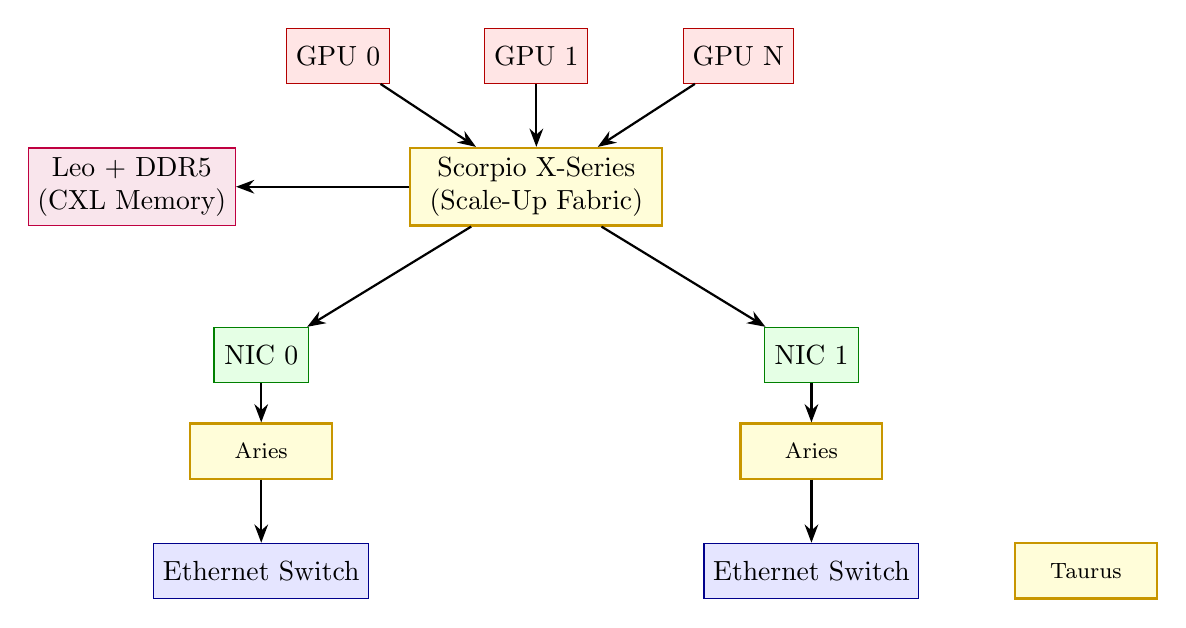
\begin{tikzpicture}[
        node distance=1.6cm and 1.2cm,
        gpu/.style={rectangle, draw=darkred, fill=red!10, minimum width=1.2cm, minimum height=0.7cm, align=center},
        nic/.style={rectangle, draw=darkgreen, fill=green!10, minimum width=1.2cm, minimum height=0.7cm, align=center},
        sw/.style={rectangle, draw=darkblue, fill=blue!10, minimum width=1.5cm, minimum height=0.7cm, align=center},
        ast/.style={rectangle, draw=gold, fill=yellow!15, thick, minimum width=1.8cm, minimum height=0.7cm, align=center},
        arrow/.style={->, >=Stealth, thick}
    ]
        \node[gpu] (GPU1) {GPU 0};
        \node[gpu, right=of GPU1] (GPU2) {GPU 1};
        \node[gpu, right=of GPU2] (GPU3) {GPU N};

        \node[ast, below=0.8cm of GPU2, minimum width=3.2cm] (SCORP) {Scorpio X-Series\\(Scale-Up Fabric)};

        \node[nic, below left=1.8cm of SCORP] (NIC1) {NIC 0};
        \node[nic, below right=1.8cm of SCORP] (NIC2) {NIC 1};

        \node[ast, below=0.5cm of NIC1, font=\footnotesize] (ARIES1) {Aries};
        \node[ast, below=0.5cm of NIC2, font=\footnotesize] (ARIES2) {Aries};

        \node[sw, below=0.8cm of ARIES1] (SW1) {Ethernet Switch};
        \node[sw, below=0.8cm of ARIES2] (SW2) {Ethernet Switch};
        \node[ast, right=of SW2, font=\footnotesize] (TAURUS_N) {Taurus};

        \node[rectangle, draw=purple, fill=purple!10, minimum width=2.5cm, minimum height=0.7cm, align=center, left=2.2cm of SCORP] (LEO_N) {Leo + DDR5\\(CXL Memory)};

        \draw[arrow] (GPU1) -- (SCORP);
        \draw[arrow] (GPU2) -- (SCORP);
        \draw[arrow] (GPU3) -- (SCORP);
        \draw[arrow] (SCORP) -- (NIC1);
        \draw[arrow] (SCORP) -- (NIC2);
        \draw[arrow] (NIC1) -- (ARIES1);
        \draw[arrow] (NIC2) -- (ARIES2);
        \draw[arrow] (ARIES1) -- (SW1);
        \draw[arrow] (ARIES2) -- (SW2);
        \draw[arrow] (SCORP) -- (LEO_N);
    \end{tikzpicture}
    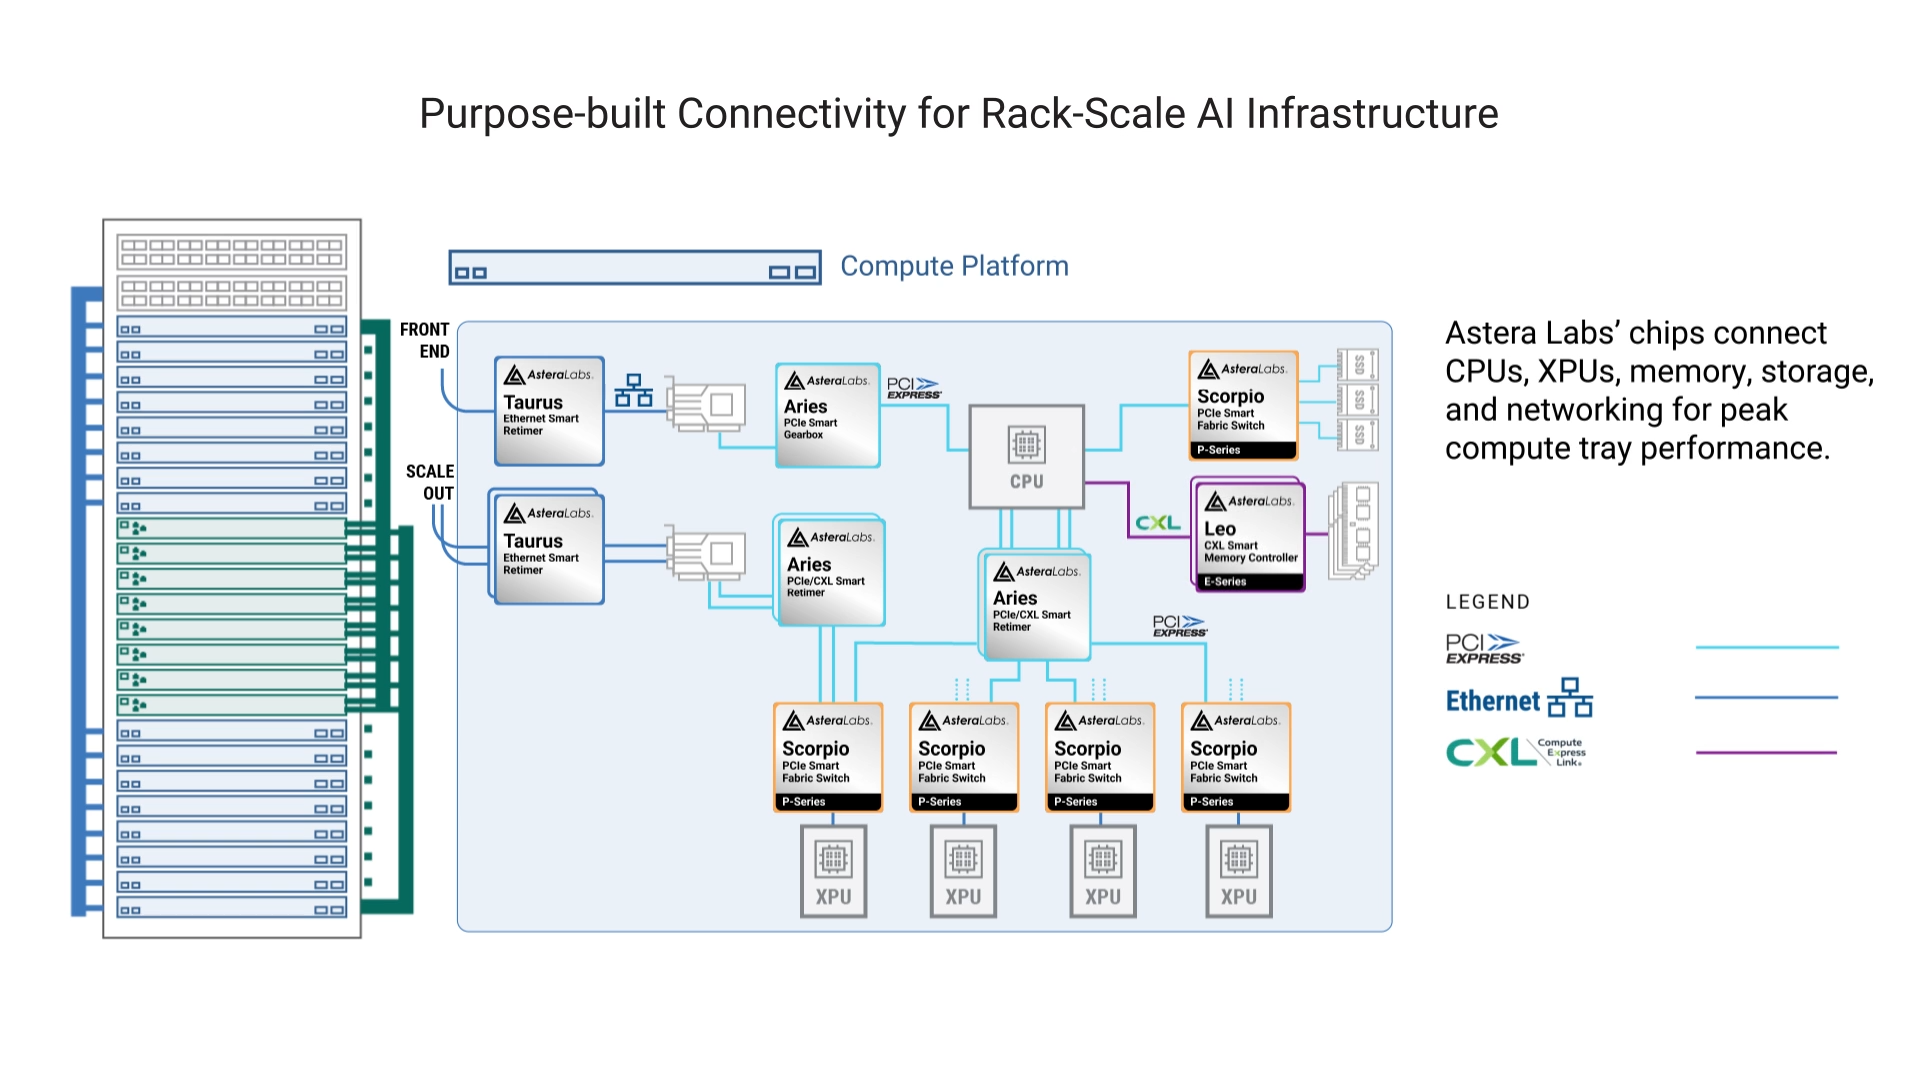
\includegraphics[width=0.9\textwidth]{./location.png}
    \caption{产品在 AI 数据中心中的物理部署位置}
    \label{fig:datacenter-location}
\end{figure}

\begin{itemize}
    \item \textbf{Scorpio X}：GPU-to-GPU Scale-Up（机箱/机架内）
    \item \textbf{Aries Retimer}：GPU/NIC 到外部连接（背板/电缆）
    \item \textbf{Taurus}：Scale-Out 网络（跨机架 Ethernet）
    \item \textbf{Leo}：CXL 内存扩展（GPU 共享内存池）
\end{itemize}


% ============================================================
%  PART 3: Scorpio 深度研究
% ============================================================
% ============================================================
%  Part 3: Scorpio 深度研究
% ============================================================

\section{Scorpio 深度研究}

\subsection{Scorpio 是什么}

Scorpio 不是传统 PCIe Switch，也不是 NVSwitch 的复制品。它是一种\textbf{新型的 Smart Fabric Switch}——基于 PCIe 6 物理层（64 GT/s PAM4）但可以运行多种协议：
标准 PCIe 6、CXL 3.x、或 memory semantic 的 platform-specific 协议。

\begin{table}[htb]
    \centering
    \caption{Scorpio 系列产品对比}
    \label{tab:scorpio}
    \begin{tabular}{lcc}
        \toprule
        \textbf{特性} & \textbf{Scorpio X-Series} & \textbf{Scorpio P-Series} \\
        \midrule
        定位 & Memory Semantic AI Fabric Switch & PCIe 6 Fabric Switch \\
        Lane Count & 320 lanes & 32–320 lanes \\
        协议 & Open \& Platform-Specific Memory Semantic & PCIe 6 / CXL 3.x \\
        目标应用 & GPU Scale-Up & 通用 I/O Fabric (GPU/NIC/NVMe) \\
        拓扑 & High-Radix, Single-Hop & 灵活 PCIe Fabric \\
        关键特性 & HW-Accelerated Collective Ops (Hypercast) & PCIe 6 Full Support \\
        出货状态 & 已出货至 Leading Hyperscalers & 已 Demo (H200 + ConnectX-8) \\
        \bottomrule
    \end{tabular}
\end{table}

Scorpio X-Series 的 320 lanes 是业界已知最大 radix 的 PCIe-based switch。
320 lanes 可以配置为 20 个 x16 端口、40 个 x8 端口、或 80 个 x4 端口。
Broadcom 的 PEX 系列公开产品最高约 144 lanes。高 radix 的核心优势是
\textbf{减少级联}：更多设备可以直接 single-hop 连接，无需多级交换级联，从而降低延迟。

\subsection{技术架构}

Scorpio 的技术分层：

\begin{enumerate}
    \item \textbf{物理层}：320$\times$ SerDes @ 64 GT/s PAM4（PCIe 6 PHY）
    \item \textbf{交换层}：High-Radix Crossbar Switch Fabric
    \item \textbf{协议引擎}：
        \begin{itemize}
            \item Standard PCIe 6 Protocol Engine（FLIT mode）
            \item Memory Semantic Protocol Engine（open + platform-specific）
        \end{itemize}
    \item \textbf{加速层}：HW-Accelerated Collective Operations (Hypercast)
    \item \textbf{管理层}：Fabric Manager via COSMOS Integration
\end{enumerate}

\textbf{关键技术参数（已确认）} \sourceT{2}：
\begin{itemize}
    \item 320 SerDes lanes @ 64 GT/s PAM4
    \item High-radix single-hop topology
    \item HW-accelerated collective ops (All-Reduce, All-to-All 等)
    \item Per-port telemetry via COSMOS
\end{itemize}

\textbf{未确认参数} \unverified{}：
\begin{itemize}
    \item 端到端转发延迟（未公开具体 ns 数）
    \item 功耗（未公开 W 数）
    \item Die size / 制程节点（未公开，推测 TSMC 7nm/5nm 级别）
\end{itemize}

\subsection{为什么 AI GPU 集群需要 Scorpio}

\textbf{场景 1：GPU Scale-Up Fabric}。多个 GPU 需要共享内存访问。NVSwitch 只支持 NVIDIA GPU。
异构集群（如混合 NVIDIA + AMD GPU 或 Google TPU + 其他加速器）需要开放替代方案。
自研 ASIC（如 Amazon Trainium、Google TPU）也需要 off-the-shelf 的 scale-up 互连方案。

\textbf{场景 2：GPU-to-NIC-to-Storage}。GPU 结果需快速写入 NVMe，或通过 NIC 发送到其他节点。
PCIe Switch 消除 CPU bottleneck——数据路径直接从 GPU 到 NIC，不经过 CPU。

\textbf{场景 3：MoE 模型通信优化}。Mixture-of-Experts 模型的每一层只有部分 expert 被激活
（例如 8 个中的 2 个），但 expert 分布在不同 GPU 上，需要频繁的 all-to-all 通信。
通信模式是``稀疏但大带宽''的——非常适合 fabric switch。
Astera Labs 官方博客（Caleb Shetland, Sr. Principal Firmware Architect）专门讨论了这个问题 \sourceT{2}。
Hypercast 技术在交换机内部对数据进行聚合（如 All-Reduce 的求和），
而非全部发到端点再计算，减少网络流量并降低延迟。
但具体的``tokens-per-watt''提升数据未公开 \unverified{}。

\textbf{场景 4：CXL 内存池}。GPU 通过 Scorpio 访问 CXL-attached DDR5 内存，
扩展有效内存容量（超越 HBM 限制）。关键 trade-off 是延迟 vs 容量。

\subsection{Scorpio vs NVSwitch 深度对比}

\begin{table}[htb]
    \centering
    \caption{Scorpio X-Series vs NVIDIA NVSwitch}
    \label{tab:scorpio-vs-nvswitch}
    \begin{tabular}{lcc}
        \toprule
        \textbf{对比维度} & \textbf{Scorpio X-Series} & \textbf{NVIDIA NVSwitch (H100/B200)} \\
        \midrule
        物理层 & PCIe 6 (64 GT/s PAM4) & NVLink 4/5 (100/200 GT/s) \\
        Per-GPU 带宽 & $\sim$128 GB/s (x16) & 900 GB/s (18 links $\times$ 50 GB/s) \\
        协议 & 开放 (PCIe/CXL) + Custom & 私有 (NVLink) \\
        GPU 兼容 & 任何 PCIe 设备 & 仅 NVIDIA GPU \\
        延迟 & 微秒级 (推测) & $<$1 微秒 \\
        Radix & 320 lanes (max) & 连接 8 GPU (DGX), 可级联 \\
        Collective Ops & HW-Accelerated (Hypercast) & SHARP (in-network compute) \\
        软件生态 & COSMOS & NVSwitch Fabric Manager \\
        \bottomrule
    \end{tabular}
\end{table}

Scorpio 在绝对带宽和延迟上无法与 NVSwitch 竞争（差距约 7$\times$ 带宽）。
其价值在于\textbf{开放性}、\textbf{异构兼容性}和\textbf{高 radix 灵活拓扑}。

NVLink/NVSwitch 带宽对比的量化理解：
\begin{itemize}
    \item NVSwitch (H100): 每个 GPU 有 18 个 NVLink 4 端口，每个 50 GB/s 双向 = 900 GB/s per GPU
    \item Scorpio via PCIe 6 x16: 64 GT/s $\times$ 16 lanes $\times$ 128/130 encoding = $\sim$128 GB/s per GPU
    \item 对于非 NVIDIA GPU（AMD MI300X PCIe、Intel Gaudi 3 PCIe），PCIe 是唯一的 scale-up 选项
    \item 即使是 H200，其 PCIe 侧也仍然是 x16 PCIe 5（64 GB/s）——在标准协议侧，Scorpio 匹配 GPU 的 PCIe 能力
\end{itemize}

\subsection{Scorpio vs Broadcom PCIe Switch}

\begin{table}[htb]
    \centering
    \caption{PCIe Fabric Switch 竞争对比}
    \label{tab:scorpio-vs-broadcom}
    \begin{tabular}{lcc}
        \toprule
        \textbf{维度} & \textbf{Scorpio (Astera)} & \textbf{PEX 系列 (Broadcom)} \\
        \midrule
        PCIe 世代 & PCIe 6 (前沿) & PCIe 5 为主, 6 roadmapped \\
        最大 lane 数 & 320 lanes & $\sim$144 lanes (公开) \\
        Memory Semantic & 支持 & 标准 PCIe only \\
        HW Collective Ops & 支持 (Hypercast) & 未知 \\
        AI 优化 & 从零为 AI 设计 & 通用数据中心 \\
        COSMOS 集成 & 原生 & 无等效平台 \\
        市场份额 & 新进入者 & 市场领导者 \sourceT{3} \\
        成熟度/稳定性 & 较新 & 极其成熟 \\
        \bottomrule
    \end{tabular}
\end{table}

Broadcom 的 PEX 系列（原 PLX Technology，2014 年被 Avago/Broadcom 收购）是行业 gold standard，
已经验证在数百万系统中，可靠性极高。Astera 的突破口在于 PCIe 6 是全新标准
（所有人都在新的起跑线上）、AI 集群的特殊需求、以及直接服务 hyperscaler 的能力。

\textbf{威胁评估}：对 Broadcom 的威胁程度为\textbf{中等}。
Scorpio 主要威胁的是 AI-specific 的增量市场，而非 Broadcom 的传统企业/存储 switch 业务。
但 AI market 的增速远超传统市场。

\subsection{Scorpio 的护城河与真实价值}

\begin{itemize}
    \item \textbf{SerDes 壁垒（最真实）}：320 lane 的 64 GT/s PAM4 SerDes 集成在一个芯片上是极大的模拟工程挑战。PAM4 的信噪比要求远高于 NRZ，crosstalk management 在 320 lane 密度下极其困难
    \item \textbf{Hyperscaler Qualification}：已通过 hyperscaler 的严格验证并出货。Qual 周期长达 12-24 个月，一旦通过更换成本高。但这只是时间壁垒，竞争对手有足够资金和时间也能通过
    \item \textbf{Memory Semantic Protocol}：可编程协议引擎的差异化是真实的，但如果竞争对手支持标准 CXL 3.x（也支持 memory semantic），功能会趋同
    \item \textbf{COSMOS 锁定}：统一管理的价值真实存在，但大型 hyperscaler 可以自己开发管理工具
\end{itemize}

\textbf{Scorpio 在 AI Infra 中的真实价值}：
目前是唯一基于 PCIe 并针对 AI 优化的大 radix fabric switch，
解决了异构 GPU 环境的 scale-up 互连问题，为 hyperscaler 提供了 NVIDIA 之外的战略性替代方案。
但其性能天花板（PCIe 带宽/延迟）限制了在最高性能场景的适用性。


% ============================================================
%  PART 4: Aries 深度研究
% ============================================================
% ============================================================
%  Part 4: Aries 深度研究
% ============================================================

\section{Aries 深度研究}

\subsection{什么是 Retimer}

Retimer 是一种信号完整性芯片，执行\textbf{完整的信号再生}而非简单的放大或均衡。
在 PCIe 6 (64 GT/s PAM4) 时代，Retimer 从``可选''变成了``必需''。

\begin{figure}[htb]
    \centering
    \begin{tikzpicture}[
        node distance=0.8cm,
        block/.style={rectangle, draw=darkblue, fill=blue!5, thick, minimum width=2cm, minimum height=0.9cm, align=center, rounded corners=3pt},
        signal/.style={->, >=Stealth, thick}
    ]
        \node[block] (TX) {TX\\发送端};
        \node[block, right=of TX] (CHANNEL) {Channel\\PCB/背板/电缆};
        \node[block, right=of CHANNEL] (RETIMER) {Retimer\\CDR + 重新驱动};
        \node[block, right=of RETIMER] (CHANNEL2) {Channel};
        \node[block, right=of CHANNEL2] (RX) {RX\\接收端};

        \draw[signal] (TX) -- (CHANNEL) node[midway, above, font=\footnotesize] {信号衰减};
        \draw[signal, darkred, very thick] (CHANNEL) -- (RETIMER) node[midway, above, font=\footnotesize] {弱/噪声信号};
        \draw[signal, darkgreen, very thick] (RETIMER) -- (CHANNEL2) node[midway, above, font=\footnotesize] {干净信号};
        \draw[signal] (CHANNEL2) -- (RX);
    \end{tikzpicture}
    \caption{Retimer 工作原理}
    \label{fig:retimer-principle}
\end{figure}

\subsubsection{Redriver vs Retimer vs DSP Retimer}

\begin{table}[htb]
    \centering
    \caption{信号调理技术对比}
    \label{tab:redriver-retimer}
    \begin{tabular}{lccc}
        \toprule
        \textbf{特性} & \textbf{Redriver} & \textbf{Analog Retimer} & \textbf{DSP Retimer (Aries)} \\
        \midrule
        功能 & 放大 + 模拟均衡 & CDR + 模拟重驱动 & CDR + DSP + 数字重驱动 \\
        时钟恢复 & 无 & 有 & 有 \\
        延迟 & $<$100 ps & 10-20 ns & 20-50 ns \\
        噪声处理 & \textbf{放大噪声} & 消除 & \textbf{完全消除} \\
        PCIe 5 & 部分可用 & 可用 & 推荐 \\
        PCIe 6 (PAM4) & \textbf{不可用} & 勉强可用 & \textbf{必需} \\
        \bottomrule
    \end{tabular}
\end{table}

PCIe 6 从 NRZ（2 电平）切换到 PAM4（4 电平），眼图开口是 NRZ 的 1/3（相同电压摆幅下）。
Redriver 的模拟均衡会同时放大信号和噪声，无法满足 PAM4 的信噪比要求。
DSP Retimer 的核心流程：CTLE（模拟前端均衡）→ ADC 数字化 → DSP（FFE/DFE/CDR/PAM4 解码/FEC）→ PAM4 编码 + DAC + Driver 输出。这个过程消除了所有累积的抖动和噪声。

\subsection{为什么 AI Server 更需要 Retimer}

传统服务器中 CPU 到 PCIe slot 距离短（$<$6 inches），通常只有 1-2 个 PCIe 设备。
AI Server 的情况完全不同：

\begin{itemize}
    \item GPU 底板面积大（$>$12 inches trace length）
    \item 8-72+ GPU per node
    \item PCIe 5/6 必需，更高 lane 数
    \item 密集 crosstalk 管理
    \item Multi-rack 需要 cable（$>$3m）
    \item 每个 GPU 需要多个 PCIe/CXL 连接
\end{itemize}

AI server 的 SI 挑战呈指数级增长：更多 GPU $\times$ 更高速度 $\times$ 更复杂拓扑 = Retimer 不可省略。
Astera Labs 声称其芯片在``80\%+ 的 AI 服务器''中使用 \sourceT{3}。
这个数字无法从官方验证 \unverified{}。

\subsection{Aries 产品线细分}

\subsubsection{Aries Smart DSP Retimer}

PCIe 6 / CXL 3.x 信号调理芯片，集成 DSP 进行 per-lane 均衡和信号再生。
与``所有主要 root complex 和 50+ endpoints''进行了互操作测试，
经过``chip-to-chip, box-to-box, rack-to-rack''拓扑的验证，配对不同 insertion loss 条件。\sourceT{2}
已与 5th Gen Intel Xeon Scalable 和 4th Gen AMD EPYC 完成互操作验证。

\subsubsection{Aries Smart Cable Module}

将 Aries DSP Retimer 集成到 cable paddle card 中。关键规格 \sourceT{2}：
\begin{itemize}
    \item \textbf{7m reach at 64 GT/s} — 被动铜缆 (DAC) 仅 3m（在 PAM4 下插入损耗极限）
    \item 细径电缆：32AWG for 4m, 27AWG for 6m — 不阻塞气流
    \item BER 显著优于 PCIe 规范要求
    \item 生态伙伴：Amphenol（OSFP-XD Gen6 AEC）、Molex（PCIe 6.0 AEC）
    \item 与 CXL 3.x 兼容
\end{itemize}

Astera 采取``inside''策略——芯片内置在 cable connector 里，终端用户看到的是 Amphenol/Molex 品牌，
但 Astera 提供端到端的固件/软件/硬件支持（``单点责任''）。

传统模式 vs Astera 模式：
\begin{itemize}
    \item 传统：客户从 Amphenol/Molex 买 cable，从 Broadcom 买 retimer，自己集成
    \item Astera：客户从 Amphenol/Molex 买``内置 Aries 的 cable''，Astera 提供统一支持
\end{itemize}

这对 hyperscaler 的价值：减少供应链复杂度、单一责任方、统一管理平面（COSMOS）。

\subsubsection{Aries Smart Gearbox}

Gearbox 是一种协议桥接芯片——一端是 PCIe 6 (64 GT/s PAM4, FLIT mode)，
另一端是 PCIe 5 (32 GT/s NRZ, TLP format)。解决的核心问题是：
Hyperscaler 有数千台已验证的 PCIe 5 NIC（如 NVIDIA ConnectX-7、Intel E810），
server 升级到 PCIe 6 CPU/GPU 后，NIC requalification 耗时 12-18 个月，
Gearbox 消除了 requal 障碍，允许增量式 PCIe 6 迁移。

Gearbox 是一个``过渡产品''——当所有 NIC 都升级到 PCIe 6 后需求会下降。
但从 PCIe 5 到 PCIe 6 的全面过渡需要 3-5 年，为 Gearbox 提供了足够的市场窗口。

\subsection{功耗/延迟/SI Trade-off}

SerDes 设计面临三重约束：

\begin{itemize}
    \item \textbf{功耗}：每代 PCIe 翻倍。PCIe 5 NRZ $\sim$300-400 mW/lane，PCIe 6 PAM4 DSP $\sim$500-700 mW/lane（推测 \speculation{}）
    \item \textbf{延迟}：DSP pipeline 深度决定延迟。更多的均衡 tap (FFE/DFE) $\to$ 更好的 SI 但更高延迟
    \item \textbf{SI 质量}：PAM4 SNR 要求远高于 NRZ，更多 DSP 处理 $\to$ 更高功耗和延迟
\end{itemize}

Astera Labs 通过自有 DSP 架构优化这个 triple trade-off，但具体数字未公开。\unverified{}
SerDes 参数通常是芯片公司最核心的商业秘密。

\subsection{竞争对比}

\begin{table}[htb]
    \centering
    \caption{PCIe Retimer/AEC 竞争格局}
    \label{tab:aries-competition}
    \begin{tabular}{lcccc}
        \toprule
        \textbf{能力} & \textbf{Astera Aries} & \textbf{Broadcom} & \textbf{Credo} & \textbf{Parade/Renesas} \\
        \midrule
        PCIe 6 支持 & \checkmark & \checkmark & \checkmark & Renesas \checkmark, Parade ? \\
        DSP Retimer & \checkmark & \checkmark & \checkmark & 部分 \\
        Smart Cable (AEC) & \checkmark（Aries SCM）& — & \checkmark（Dove AEC）& — \\
        Gearbox & \checkmark & — & — & — \\
        COSMOS 集成 & \checkmark & — & — & — \\
        Hyperscaler 直接关系 & 强 & 强（通过 OEM）& 中强 & 弱 \\
        \bottomrule
    \end{tabular}
\end{table}

在\textbf{retimer 单一产品}上，Astera/Broadcom/Credo 都有竞争力。
Astera 的优势在于\textbf{全栈集成}：Retimer + Cable + Gearbox + Switch + CXL + Software。
Credo 在 AEC 市场有先发优势（Dove 系列是最知名的 PCIe AEC），Astera 在后追赶但增速快。
Credo 的最大优势在于低功耗 SerDes IP。

\subsection{技术优势评估}

Astera Labs 在 Aries 领域的技术评估：
\begin{itemize}
    \item \textbf{已验证的优势}：PCIe 6 DSP Retimer 出货（时间先发）、50+ endpoint 互操作验证、Smart Cable 集成 DSC telemetry
    \item \textbf{可能为营销} \marketing{}：声称 BER``显著优于''PCIe 规范——在没有具体测试条件的情况下无法验证；``industry-leading 7m reach''——Credo 也有类似能力
    \item \textbf{无法确认} \unverified{}：具体功耗/延迟数据、具体 ASP/margin、市场份额
\end{itemize}


% ============================================================
%  PART 5: Leo 与 CXL
% ============================================================
% ============================================================
%  Part 5: Leo 与 CXL
% ============================================================

\section{Leo 与 CXL}

\subsection{什么是 CXL}

CXL（Compute Express Link）是基于 PCIe 物理层构建的\textbf{缓存一致性}互连协议。
允许 CPU/GPU 以 load/store 语义直接访问远端内存和外设。

CXL 有三种协议类型：
\begin{enumerate}
    \item \textbf{CXL.io}：基于 PCIe，用于设备发现、配置、寄存器访问（必须支持）
    \item \textbf{CXL.cache}：允许设备访问 host CPU 的缓存（用于加速器）
    \item \textbf{CXL.mem}：允许 host 访问设备上的内存（用于内存扩展）
\end{enumerate}

Leo 属于 Type 3 设备：支持 CXL.io + CXL.mem，不支持 CXL.cache。
这意味着 Leo 是一个``被动''的内存设备——CPU 可以访问 Leo 管理的内存，
但 Leo 不会主动访问 CPU 缓存。

\begin{table}[htb]
    \centering
    \caption{CXL 标准演进时间线}
    \label{tab:cxl-evolution}
    \begin{tabular}{llll}
        \toprule
        \textbf{版本} & \textbf{发布时间} & \textbf{PHY 带宽} & \textbf{关键特性} \\
        \midrule
        CXL 1.0/1.1 & 2019/2020 & PCIe 5 (32 GT/s) & Type 3 内存设备, 单 host \\
        CXL 2.0 & 2020 & PCIe 5 & Switching, Memory Pooling (多 host) \\
        CXL 3.0 & 2022 & PCIe 6 (64 GT/s) & Memory Sharing (多 host 同时), GFAM \\
        CXL 3.1/3.2 & 2023/2024 & PCIe 6 & 3.x 优化 \\
        CXL 4.0 & 2025 年 11 月 & 128 GT/s & 242 GB/s per x16 \\
        \bottomrule
    \end{tabular}
\end{table}

\subsection{Memory Wall}

Memory Wall（内存墙）是指计算速度与内存访问速度之间的差距持续扩大。
历史上（1986-2000）：CPU 速度年增 55\%，而 off-chip 内存响应时间年增仅 10\%。

在 AI 训练/推理场景中的具体表现：
\begin{itemize}
    \item H100 GPU 计算吞吐：$\sim$2000 TFLOPS (FP8)；HBM3 带宽：3.35 TB/s
    \item 算术密度：$\sim$0.6-1.5 Bytes/FLOP；HBM 提供 3.35 TB/s / 2000 TFLOPS = 1.675 Bytes/FLOP（勉强匹配）
    \item 但如果模型参数超过 HBM 容量（80GB），需要外部访问：PCIe 5 x16 仅 64 GB/s
    \item 64 GB/s / 2000 TFLOPS = 0.032 Bytes/FLOP——差了 50$\times$！
\end{itemize}

\textbf{Training 场景}：大模型（$>$100B 参数）的 weights/optimizer states/gradients 远超单 GPU HBM，
需要跨 GPU 共享。CXL 扩展 DDR5 可以放 optimizer states、embeddings 等不频繁访问的数据，
但不适合放频繁更新的 weights（延迟太高）。

\textbf{Inference 场景}（CXL 更具价值）：
KV cache 是主要内存消耗（长上下文可达 TB 级），
对延迟容忍度高（prefill/decode 的计算时间远大于 CXL 延迟）。
CXL DDR5 可以在 TB 级别提供 KV cache 容量，成本远低于增加 GPU。

\textbf{RAG 场景}：向量数据库/知识库需要大容量内存，CXL 提供比网络存储低得多的访问延迟。
Astera Labs 博客专门讨论了``CXL for RAG and KV Cache Performance''。\sourceT{2}

\subsection{Memory Expansion vs Pooling vs Sharing}

\begin{table}[htb]
    \centering
    \caption{CXL 内存架构三种模式}
    \label{tab:cxl-modes}
    \begin{tabular}{lccc}
        \toprule
        \textbf{特征} & \textbf{Memory Expansion} & \textbf{Memory Pooling} & \textbf{Memory Sharing} \\
        \midrule
        架构 & 1 host : 1 CXL 设备 & N host : 1 pool (switch) & N host : 1 memory (coherent) \\
        所需 CXL 版本 & 1.1+ & 2.0+ & 3.0+ \\
        带宽 & 全 CXL 链路带宽 & 通过 switch 共享 & 共享，coherency 开销 \\
        主要价值 & 增加单机内存容量 & 减少 stranded memory & 真正的 disaggregation \\
        复杂度 & 低 & 中 & 极高 \\
        延迟 & 最低（直连） & 中（经过 switch） & 中高（coherency protocol） \\
        \bottomrule
    \end{tabular}
\end{table}

\subsection{Leo CXL Memory Controller}

\begin{table}[htb]
    \centering
    \caption{Leo 技术规格（来源：官方 interop 报告 \sourceT{2}）}
    \label{tab:leo-specs}
    \begin{tabular}{ll}
        \toprule
        \textbf{参数} & \textbf{已知值} \\
        \midrule
        CXL 版本 & CXL 1.1 \\
        内存类型 & DDR5-5600 RDIMM \\
        已验证容量 & 64GB RDIMM (Micron/Samsung/SK hynix) \\
        CPU 兼容 & Intel Xeon 6, AMD EPYC \\
        OS 支持 & Linux \\
        软件 & COSMOS for telemetry/RAS \\
        \midrule
        \textbf{未公开参数} & \textbf{状态} \\
        \midrule
        每控制器最大内存容量 & \unverified{} 未公开 \\
        内存通道数 & \unverified{} 未公开 \\
        CXL 链路带宽 & \unverified{} 未公开（推测 PCIe 5 x8 或 x16） \\
        Read/Write 延迟 & \unverified{} 未公开 \\
        功耗 & \unverified{} 未公开 \\
        \bottomrule
    \end{tabular}
\end{table}

Leo 当前支持 CXL 1.1（根据官网 interop 报告）。
CXL 1.1 不支持 switching（一个 host 只能连接一个 Type 3 设备），
不支持多 host 共享（memory sharing 需要 CXL 3.0）。
这意味着 Leo 目前只能做``memory expansion''（1 对 1），不能做``memory pooling''（多对多）。

\textbf{竞争对比}（CXL 内存控制器供应商）：
\begin{itemize}
    \item Samsung：128GB/512GB CXL 内存模块，自研控制器（垂直整合模式）
    \item SK hynix：CXL 内存方案
    \item Montage Technology：MXC GEN3, CXL 内存控制器
    \item Micron：CXL fabric memory sharing demo
    \item Astera Labs Leo：独立控制器芯片（不卖内存模块，赋能内存模组厂商模式）
\end{itemize}

关键区别：Astera 只卖控制器芯片，不卖内存模块。Samsung/SK hynix 卖的是完整的内存模块（控制器 + DRAM）。
Astera 的模式是赋能内存模组厂商，让 A-Data, Kingston, SMART Modular 等可以做出兼容的 CXL 内存模块。

\subsection{CXL 当前真实的落地情况}

\begin{table}[htb]
    \centering
    \caption{CXL 落地状态评估（截至 2026 年中）}
    \label{tab:cxl-status}
    \begin{tabular}{lp{0.5\textwidth}}
        \toprule
        \textbf{状态} & \textbf{详情} \\
        \midrule
        \checkmark 已实现 & CPU 支持（Intel SR/GR/XR、AMD Genoa）、OS 支持（Linux 6.5+、Win Server 2022）、合规程序（Integration List）、CXL 4.0 spec 发布 \\
        \checkmark 部分实现 & Demo（SC24/SC25 多个 CXL demo）、MXC GEN3 硅片可用 \\
        $\times$ 未实现 & 大规模生产部署、CXL 3.0 memory sharing 量产硅片、标准化内存模块格式 \\
        \bottomrule
    \end{tabular}
\end{table}

\textbf{CXL 距离大规模生产部署可能还需要 2-4 年}。当前的部署主要是 hyperscaler 的有限试验。
Memory expansion (1:1) 比 pooling/sharing 更接近生产就绪。

\textbf{主要障碍}：
\begin{enumerate}
    \item \textbf{延迟}：CXL 控制器增加 $\sim$200ns 延迟——对延迟敏感应用不适合
    \item \textbf{软件生态}：Memory tiering（hot/cold page 管理）、Fabric Manager 仍在成熟中
    \item \textbf{成本}：CXL 内存模块比标准 DDR5 DIMM 贵 20-50\%（估计）
    \item \textbf{带宽竞争}：Pooling 场景下多 host 共享带宽，产生 contention
    \item \textbf{一致性复杂度}：CXL 3.0+ 的 multi-host cache coherency 验证极其困难
\end{enumerate}

对 Astera Labs 来说，Leo 是面向未来的战略性投资。短期内（1-2 年）Leo 的收入贡献可能有限，
但如果 CXL adoption 加速（2027-2028），Leo 将成为重要增长引擎。


% ============================================================
%  PART 6: COSMOS 软件平台
% ============================================================
% ============================================================
%  Part 6: COSMOS 软件平台
% ============================================================

\section{COSMOS 软件平台}

\subsection{COSMOS 是什么}

COSMOS = \textbf{CO}nnectivity \textbf{S}ystem \textbf{M}anagement and \textbf{O}ptimization \textbf{S}oftware。
是 Astera Labs Intelligent Connectivity Platform 的软件层。\sourceT{2}

\begin{figure}[htb]
    \centering
    \begin{tikzpicture}[
        node distance=1cm,
        layer/.style={rectangle, draw=darkblue, fill=blue!5, thick, minimum width=6cm, minimum height=0.8cm, align=center, rounded corners=3pt},
    ]
        \node[layer, fill=darkgreen!10] (APP) {COSMOS Tools (CLI + Explorer GUI)};
        \node[layer, below=0.2cm of APP] (SDK) {COSMOS Developer Kit (SDK + 库 + 脚本)};
        \node[layer, below=0.2cm of SDK] (CORE) {COSMOS Core Platform};
        \node[layer, fill=darkblue!15, below=0.2cm of CORE] (LINK) {Link Management（链路监控/诊断/优化）};
        \node[layer, fill=darkblue!15, below=0.2cm of LINK] (FLEET) {Fleet Management（Rack-Scale 资源管理）};
        \node[layer, fill=darkblue!15, below=0.2cm of FLEET] (RAS) {RAS Management（可靠性/可用性/可服务性）};
        \node[layer, fill=darkred!10, below=0.2cm of RAS] (HW) {Scorpio + Aries + Leo + Taurus 硬件};
    \end{tikzpicture}
    \caption{COSMOS 平台架构}
    \label{fig:cosmos-arch}
\end{figure}

\subsection{COSMOS 的三个功能支柱}

\subsubsection{Link Management}

Per-lane level 的 PCIe/CXL 链路监控。提供：
\begin{itemize}
    \item 数千条数据链路的实时性能监控
    \item Per-lane signal quality metrics
    \item 温度读数 per link
    \item 链路稳定性验证和诊断
\end{itemize}

\subsubsection{Fleet Management}

跨数千节点的 rack-scale 资源管理和优化。为 hyperscale 数据中心的
``rack-scale deployment'' 设计，管理 compute power、efficiency、TCO 的平衡。

\subsubsection{RAS Management}

Reliability, Availability, Serviceability —— 预测性故障分析：
\begin{itemize}
    \item 预测故障发生的时间和位置
    \item 主动隔离故障点
    \item 目标：最大化系统可用性（uptime）
\end{itemize}

\subsection{为什么 Connectivity Chip 公司需要软件平台}

\textbf{硬件差异化越来越难维持}：PCIe retimer/switch 在任何市场上都有多个供应商，
硬件的性能差异随时间缩小。软件平台创造的是``改用成本''（switching cost）。

\textbf{Hyperscaler 的操作需求}：管理 100,000+ 节点的连接健康状态不能靠人工，需要自动化。
COSMOS 提供``单一管理平面''——不管用 Scorpio/Aries/Leo/Taurus，都是同一个 API。

\textbf{成本视角}（推测 \speculation{}）：
一个 Aries Retimer 芯片成本 $\sim$\$50-100，
一个 DGX H100 节点成本 $\sim$\$300,000，
一个 training cluster 成本 $\sim$\$100M+。
如果一个 \$50 的芯片故障导致 \$100M 的 cluster downtime，
连接可靠性就不再是``锦上添花''而是``关键任务''。
这就是 telemetry 和预测性故障检测的核心价值。

\subsection{COSMOS vs NVIDIA Fabric Manager}

\begin{table}[htb]
    \centering
    \caption{AI 集群管理平台对比}
    \label{tab:cosmos-vs-nvidia}
    \begin{tabular}{lcc}
        \toprule
        \textbf{能力} & \textbf{COSMOS (Astera)} & \textbf{NVIDIA Fabric Manager} \\
        \midrule
        管理范围 & 跨品牌、跨协议的连接设备 & 仅 NVLink/NVSwitch \\
        Telemetry 深度 & Per-lane signal quality & NVLink level \\
        预测性故障 & 支持 & 支持 (DGX) \\
        开放 API & 提供 SDK & 部分开放 \\
        协议覆盖 & PCIe + CXL + Ethernet & NVLink only \\
        Fleet scale & Hyperscaler rack-scale & DGX/SuperPOD scale \\
        第三方硬件支持 & 任何 PCIe/CXL 设备 & 仅 NVIDIA \\
        \bottomrule
    \end{tabular}
\end{table}

COSMOS 的核心差异化：\textbf{跨厂商、跨协议的连接管理}。NVIDIA 管理 NVLink，
COSMOS 管理除此之外的一切。两者不是竞争关系，而是互补——
尤其是在包含 NVIDIA GPU 的异构集群中。

\subsection{软件是否会成为 Astera Labs 的护城河}

\textbf{短期（1-3 年）——有效的差异化}：
竞争对手（Broadcom、Credo）没有类似平台。Hyperscaler 一旦将 COSMOS API 集成到自己的管理系统，
更换成本高。提供全套硬件 + 软件支持也使得 Astera 对资源紧张的 hyperscaler 团队更有吸引力。

\textbf{长期（3-5 年）——不确定}：
有能力的 hyperscaler 可以自己开发类似的管理软件（Google、Amazon 已在做）。
对软件能力弱的客户，COSMOS 的锁定效应更强。
开源替代可能涌现（类似 OpenBMC 管理 BMC 的方式）。
最大的竞争风险：NVIDIA 可能将 Fabric Manager 扩展到 PCIe 域（如果 NVIDIA 自研 PCIe switch）。

\textbf{商业模式意义}：硬件售卖是一次性收入（虽然 hyperscaler 会持续采购），
软件支持/更新可以产生 recurring 收入（类似 Cisco 的 SmartNet 模式）。
目前 Astera 尚未明确收费模式，但长期看软件可能是高毛利 recurring revenue 来源。


% ============================================================
%  PART 7: 技术壁垒分析
% ============================================================
% ============================================================
%  Part 7: 技术壁垒分析
% ============================================================

\section{技术壁垒分析}

\subsection{护城河全景评估}

\begin{table}[htb]
    \centering
    \caption{Astera Labs 技术壁垒强度评估}
    \label{tab:moat}
    \begin{tabular}{lccp{0.3\textwidth}}
        \toprule
        \textbf{壁垒} & \textbf{强度} & \textbf{持久性} & \textbf{被复制的难度} \\
        \midrule
        \rowcolor{t1green}
        高速 SerDes (320-lane PAM4) & \checkmark\checkmark\checkmark & 中 & 极高——模拟设计需多年积累 \\
        \rowcolor{t2blue}
        Hyperscaler Qualification & \checkmark\checkmark\checkmark & 中短 & 高——时间 + 资源壁垒 \\
        \rowcolor{t3yellow}
        PCIe/CXL Interop 验证 & \checkmark\checkmark & 中 & 中——需要大量设备和时间 \\
        \rowcolor{t3yellow}
        Memory Semantic Protocol & \checkmark\checkmark & 短中 & 中——其他厂商可开发 \\
        \rowcolor{t4orange}
        COSMOS 软件生态 & \checkmark\checkmark & 短中 & 中低——可自研或开源替代 \\
        \rowcolor{t4orange}
        ``Switzerland'' 中立性 & \checkmark & 短 & 低——随竞争格局变化 \\
        \rowcolor{t4orange}
        专利组合 & 未知 & 未知 & 未知——需专利检索 \unverified{} \\
        \bottomrule
    \end{tabular}
\end{table}

\subsection{真实壁垒详解}

\subsubsection{高速 SerDes（最真实、最深的技术壁垒）}

320 个 64 GT/s PAM4 lane 在一个芯片上的信号完整性管理是极端挑战。
每个 lane 需要 CTLE + DFE + CDR + PAM4 decoder。
320 lane $\times$ $\sim$600 mW/lane = $\sim$192W 仅用于 SerDes（还不包括 switch fabric）。
Crosstalk management 在 320 lane 密度下极其困难。

SerDes 团队需要 10+ 年经验，全球范围内人才极其稀缺。但这不是不可逾越的——Broadcom、Marvell、Intel 都有 SerDes 能力。

\subsubsection{Hyperscaler Qualification（时间壁垒）}

Qual 周期包括：热冲击测试、加速老化、FIT rate 验证、电源噪声测试、系统级互操作测试。
周期长达 12-24 个月。一旦通过，更换成本高。
但这是时间壁垒而非技术壁垒——竞争对手如果有决心和资金，可以跨越。
Hyperscaler 的``second source''策略反而保护了 Astera——他们需要至少两个供应商。

\subsubsection{PCIe/CXL Interop 验证（生态壁垒）}

与所有主要 host（Intel, AMD, ARM）、memory（Micron, Samsung, SK hynix）、
GPU（NVIDIA, AMD）的互操作需要巨大的测试实验室和持续投入。
New comer 需做同样的投入。这构成了中等等级的生态壁垒。

\subsubsection{COSMOS（软件壁垒，中等但脆弱）}

软件创造的锁定效应是真实的，但大型 hyperscaler 可以自研。
关键是：hyperscaler 愿意``外包''多少软件能力给芯片供应商？
这取决于 (1) 供应商的软件质量 (2) hyperscaler 自身的软件团队规模。

\subsection{哪些壁垒可能被侵蚀}

\textbf{最大威胁：Broadcom 的 AI 优化 PCIe 6 Switch}。
Broadcom 拥有全球最强的 SerDes 团队之一，已有 PCIe switch 的客户关系和生态。
如果 Broadcom 推出 320-lane AI-optimized PCIe 6 switch，
Scorpio 的差异化会大幅缩小。时间线是主要变量。

\textbf{第二威胁：NVIDIA 扩展管理平台到 PCIe 域}。
如果 NVIDIA 自研 PCIe switch，会与 NVSwitch 形成完整 AI 互连栈。
NVIDIA 有动机（增加 GPU 销售）、能力（SerDes/芯片设计）、客户关系。
但 NVIDIA 这样做会进一步加深客户锁定 → hyperscaler 会抵制。
这是个 tension：NVIDIA 的能力 vs hyperscaler 的意愿。

\textbf{第三威胁：Credo 在 AEC 市场的先发优势}。
Credo 在 AEC 市场比 Astera 早多年进入，Astera 在 AEC 领域是后来者。

\textbf{长期视角}：市场可能收敛到 2-3 家供应商。
Astera 的生存取决于：(1) 产品代际领先 (2) COSMOS 锁定 (3) hyperscaler 的 multi-source 策略。
``被吃掉''可能不是 Broadcom/NVIDIA 的收购，而是市场份额的侵蚀。


% ============================================================
%  PART 8: 竞争格局
% ============================================================
% ============================================================
%  Part 8: 竞争格局
% ============================================================

\section{竞争格局}

\subsection{全面竞争矩阵}

\begin{table}[htb]
    \centering
    \caption{竞争格局矩阵 (2026)}
    \label{tab:competition-matrix}
    \small
    \begin{tabular}{lccccc}
        \toprule
        \textbf{公司} & \textbf{Retimer} & \textbf{PCIe Switch} & \textbf{CXL Ctrl} & \textbf{AEC} & \textbf{软件} \\
        \midrule
        \rowcolor{blue!10}
        \textbf{Astera Labs} & \checkmark\checkmark\checkmark & \checkmark\checkmark\checkmark & \checkmark\checkmark & \checkmark\checkmark & \checkmark\checkmark\checkmark \\
        Broadcom & \checkmark\checkmark & \checkmark\checkmark\checkmark & — & \checkmark & — \\
        NVIDIA & 自用 & 私有(NVSwitch) & 间接 & — & 自用 \\
        Credo & \checkmark\checkmark\checkmark & — & — & \checkmark\checkmark\checkmark & — \\
        Marvell & \checkmark & 定制 ASIC & — & \checkmark & — \\
        Microchip & — & \checkmark\checkmark & \checkmark & — & — \\
        Samsung & — & — & \checkmark\checkmark\checkmark & — & — \\
        SK hynix & — & — & \checkmark\checkmark\checkmark & — & — \\
        Montage & — & — & \checkmark\checkmark & — & — \\
        Synopsys & — & — & (IP 授权) & — & — \\
        Intel & 自用 & 间接 & 自用(CPU 侧) & — & 部分 \\
        AMD & 自用 & 间接 & 自用(CPU 侧) & — & 部分 \\
        \bottomrule
    \end{tabular}
\end{table}

\subsection{分层竞争分析}

\subsubsection{Direct Competitors}

\begin{itemize}
    \item \textbf{Broadcom}：PCIe switch + retimer。最全面、最强的直接竞争对手。PEX 系列市场领导者，拥有十多年积累和客户关系
    \item \textbf{Credo}：AEC + retimer。在 AEC 市场是最大威胁，以低功耗 SerDes 著称
    \item \textbf{Samsung/SK hynix/Montage}：CXL memory controller。与 Leo 直接竞争
\end{itemize}

\subsubsection{部分竞争}

\begin{itemize}
    \item \textbf{Marvell}：数据中心芯片（DPU、定制 ASIC），不精确重叠但在同一个客户预算池中竞争
    \item \textbf{Microchip}：PCIe switch（Switchtec 系列），但在 AI 优化方面落后
\end{itemize}

\subsubsection{生态伙伴（非竞争）}

\begin{itemize}
    \item \textbf{Intel/AMD}：CPU 供应商，CXL 生态推动者，Astera 的互操作伙伴
    \item \textbf{Synopsys/Cadence}：IP 供应商，提供 SerDes/CXL IP 但不卖芯片
    \item \textbf{NVIDIA}：既是竞争（NVSwitch vs Scorpio）又是合作（COSMOS 管理 GPU 的 PCIe 侧）
\end{itemize}

\textbf{关键空白区域}：没有任何一家竞争对手覆盖 Astera 的全部产品线。
这是 Astera ``全栈''策略的核心优势。但这也意味着 Astera 同时与多家公司竞争。

\subsection{``Switzerland of Connectivity'' 定位分析}

这个定位的前提条件包括：
\begin{enumerate}
    \item GPU 市场不是 NVIDIA 垄断（需要有 AMD、Intel、自研 ASIC 等替代品）
    \item Hyperscaler 维持多 vendor 策略
    \item 开放标准（PCIe/CXL）继续成为主流连接方式
    \item NVIDIA 不将 NVLink 开放为标准
\end{enumerate}

当前这些前提条件的状态：
\begin{itemize}
    \item NVIDIA 在 AI GPU 市场 $>$80\% 份额 → 中立性对 hyperscaler 很重要但 TAM 受限
    \item Hyperscaler 确实在推多 vendor 策略（Google TPU、Amazon Trainium、MS Maia）→ 利好
    \item PCIe/CXL 持续演进 → 利好
    \item NVIDIA 未开放 NVLink → 利好
\end{itemize}

\textbf{风险}：在极端情况下——比如 NVIDIA 完全开放 NVLink 或收购一家连接公司——这个定位会迅速失效。

\subsection{Why Hyperscaler 不愿完全绑定 NVIDIA}

\begin{enumerate}
    \item \textbf{定价权}：NVIDIA GPU 的议价能力已让 hyperscaler 极度不安
    \item \textbf{供应安全}：单供应商风险（尽管 NVIDIA 已多源 HBM/制造）
    \item \textbf{技术路线自主}：Hyperscaler 希望对硬件架构有控制权
    \item \textbf{定制化需求}：通用 GPU 无法满足所有场景，需要异构计算
    \item \textbf{NVLink 锁定}：NVLink 的封闭生态是 hyperscaler 最不想看到的长尾风险——使用 NVLink 意味着整个硬件栈被 NVIDIA 绑定
\end{enumerate}

Astera Labs 的存在价值与 NVIDIA 的垄断程度\textbf{正相关}。
NVIDIA 越封闭 → Astera 越有价值。但 paradoxically，
Astera 的短期最大客户可能是 NVIDIA GPU 集群中的连接需求。
(因为 NVIDIA GPU 也需要 PCIe retimer/switch 来连接 NIC、NVMe 等非 NVLink 设备。)


% ============================================================
%  PART 9: 财务与商业分析
% ============================================================
% ============================================================
%  Part 9: 财务与商业分析
% ============================================================

\section{财务与商业分析}

\subsection{收入与增长}

以下财务数据来源于 SEC EDGAR XBRL API（CIK: 0001736297），属于 T1 级别可验证信息。

\begin{table}[htb]
    \centering
    \caption{Astera Labs 季度收入}
    \label{tab:revenue}
    \begin{tabular}{lcc}
        \toprule
        \textbf{期间} & \textbf{收入} & \textbf{说明} \\
        \midrule
        Q1 2025 (结束于 Mar 2025) & \$159.4M & \sourceT{1} 10-Q \\
        Q2 2025 (结束于 Jun 2025) & \$191.9M & \sourceT{1} 10-Q \\
        Q3 2025 (结束于 Sep 2025) & \$230.6M & \sourceT{1} 10-Q \\
        Q4 2025 (结束于 Dec 2025) & \$270.6M & \sourceT{1} 10-K (推算) \\
        \rowcolor{blue!8}
        \textbf{FY2025 全年} & \textbf{\$852.5M} & \sourceT{1} 10-K \\
        \midrule
        Q1 2026 (结束于 Mar 2026) & \$308.4M & +\textbf{93\% YoY} \sourceT{1} 10-Q \\
        \bottomrule
    \end{tabular}
\end{table}

季度收入连续增长：Q1→Q2 (+20\%)、Q2→Q3 (+20\%)、Q3→Q4 (+17\%)。
Q1 2026 年化收入约 \$1.23B。与历史收入（2022 年 $\sim$\$80M, 2023 年 $\sim$\$116M）对比，
3 年间增长约 10 倍，由 AI 数据中心建设推动。\sourceT{2}\sourceT{3}

增长驱动力（来自官方 Q1 2026 财报声明）：``PCIe 6 AI fabric and signal conditioning portfolio''。\sourceT{2}

\subsection{利润率分析}

\begin{table}[htb]
    \centering
    \caption{利润指标分析}
    \label{tab:margins}
    \begin{tabular}{lcccc}
        \toprule
        \textbf{期间} & \textbf{毛利率} & \textbf{净收入} & \textbf{净利率} \\
        \midrule
        Q2 2025 & 75.9\% & \$51.2M & 26.7\% \\
        Q3 2025 & 76.2\% & \$91.1M & 39.5\% \\
        \rowcolor{blue!8}
        FY2025 全年 & $\sim$75.7\% & \$219.1M & 25.7\% \\
        Q1 2026 & $\sim$76.2\% & \$80.3M & 26.0\% \\
        \bottomrule
    \end{tabular}
\end{table}

75\%+ 的毛利率在 fabless 半导体行业中属于极高水平。
行业对比：NVIDIA 75-78\%, Broadcom 65-70\%, Credo $\sim$60\%, Marvell $\sim$60\%+。\sourceT{3}
Astera 的 75\%+ 毛利率接近 NVIDIA 水平——对一个``连接件''公司来说是非常高的定价权体现。

如此高的毛利率会吸引更多竞争。随着竞争加剧和产品成熟，毛利率可能承压。
未来毛利率趋势取决于 Scorpio 的定价权和 Aries 的竞争格局。

\subsection{客户集中度}

Amazon 是已知的第一个大客户（来自 SemiAnalysis \sourceT{3}）。其他 hyperscaler 客户未公开。
推测前 2-3 大客户可能占总收入 $>$50\%。单一 hyperscaler 的采购决策会显著影响收入——
这是重大风险。需要关注 Astera 的客户 diversification 进展。\sourceT{3}

\subsection{TAM 与增长驱动}

\textbf{增长驱动}：
\begin{enumerate}
    \item AI GPU 出货量增长：每多一个 GPU，就需要更多 retimer/switch/cable
    \item GPU 密度增长：每节点 GPU 数从 8→16→72+，连接数指数级增长
    \item PCIe 6 adoption：每代 PCIe 升级都创造新的 retimer 需求（Redriver 无法处理 PAM4）
    \item Multi-rack GPU clustering：机架间连接需要 Smart Cable（$>$3m reach）
    \item CXL adoption：如果 CXL 起飞，TAM 扩展
\end{enumerate}

\textbf{TAM 估计}（置信度：中低——AI connectivity 细分市场太新，Gartner/IDC 尚无详细报告）：
\begin{itemize}
    \item PCIe Retimer (AI)：数亿美元/年
    \item PCIe Switch (AI)：数亿-十亿美元/年
    \item CXL Controller：数亿美元/年（潜在，取决于 CXL adoption）
    \item Smart Cable Module：数亿美元/年
\end{itemize}

\begin{warningblock}
{\color{darkred}\textbf{Note}}：上述 TAM 数字为基于已知信息的估算，非直接来自第三方报告。AI connectivity 细分 TAM 是一个快速移动的目标。
\end{warningblock}

\subsection{风险评估}

\begin{table}[htb]
    \centering
    \caption{Astera Labs 主要风险因素}
    \label{tab:risks}
    \begin{tabular}{lcc}
        \toprule
        \textbf{风险} & \textbf{严重性} & \textbf{可能性} \\
        \midrule
        \rowcolor{red!10}
        客户集中度（前 3 大可能 $>$50\% 收入）& 极高 & 确定存在 \\
        \rowcolor{red!10}
        AI CAPEX 周期依赖 & 极高 & 中——AI 投资是否可持续？ \\
        \rowcolor{orange!10}
        Broadcom 推出竞争产品 & 高 & 高——几乎确定 \\
        \rowcolor{orange!10}
        NVIDIA 扩展连接产品线 & 高 & 中 \\
        \rowcolor{orange!10}
        毛利率压力（竞争加剧）& 高 & 中高——随时间增加 \\
        \rowcolor{orange!5}
        CXL adoption 速度慢于预期 & 中 & 高 \\
        \rowcolor{yellow!10}
        技术代际风险（PCIe 7 / 光学互连）& 中 & 低中 \\
        \rowcolor{yellow!10}
        供应链中断（TSMC 依赖）& 中 & 低 \\
        \bottomrule
    \end{tabular}
\end{table}

\textbf{最大风险详解}：

客户集中度（最被低估的风险）：如果前 2 大客户占收入 60-70\%，
任何一个的采购决策变化都会导致收入大幅波动。

AI CAPEX 周期（最系统性风险）：AI infrastructure 的投入是周期性的（尽管当前是上升周期）。
如果 AI 投资回报不及预期 → AI CAPEX 削减 → 直接影响 Astera。

Broadcom 的威胁（最直接的竞争风险）：Broadcom 的资源和规模远超 Astera。
如果 Broadcom 认真投入 AI PCIe connectivity，可以在 2-3 年内推出有竞争力的产品。
但 Broadcom 有很多业务线，AI PCIe switch 可能不是最优先的。

\subsection{估值与市场观点}

\textbf{为什么市场给高估值}：
\begin{itemize}
    \item AI 基础设施中共识性的``瓶颈''领域——connectivity
    \item 高增长（+93\% YoY）+ 高毛利（75\%+）+ 正盈利（26\% net margin）
    \item 全栈平台比单一产品公司享有更高估值
    \item ``NVIDIA ecosystem play''的溢出效应——投资者寻找 NVIDIA 之外的 AI infra 投资标的
\end{itemize}

\textbf{市场最担心的}：
\begin{itemize}
    \item 客户集中度 → 收入脆弱性
    \item Broadcom 的进入 → 竞争格局恶化
    \item AI 投资周期 → 增长可持续性
    \item Scorpio 的 TAM 规模 → 这是最大的估值变量
\end{itemize}

\textbf{长期增长持续性} \speculation{}：
如果 Scorpio 成为 AI GPU scale-up 的事实标准 → 巨大的长期价值。
如果 Scorpio 只在 niche 市场成功 → 增长可能很快触顶。
Bull case: LTM 收入 3-5 年内达到 \$5B+, 70\%+ 毛利。
Bear case: Broadcom 快速跟进，增长受阻。


% ============================================================
%  PART 10: 最终总结
% ============================================================
% ============================================================
%  Part 10: 最终总结
% ============================================================

\section{最终总结}

\subsection{十大维度综合评估}

\begin{table}[htb]
    \centering
    \caption{综合评估总结}
    \label{tab:final-assessment}
    \begin{tabular}{lp{0.5\textwidth}}
        \toprule
        \textbf{维度} & \textbf{评估} \\
        \midrule
        \rowcolor{darkgreen!10}
        核心价值 & AI 基础设施中不可替代的连接层供应商 \\
        \rowcolor{darkgreen!10}
        最核心技术优势 & 320-lane 64 GT/s PAM4 SerDes + 全栈连接平台 \\
        \rowcolor{darkgreen!5}
        最强产品 & Scorpio X-Series（独特定位，极少直接竞争） \\
        \rowcolor{orange!10}
        最脆弱点 & 客户集中度 + Broadcom 的潜在竞争威胁 \\
        \rowcolor{darkgreen!5}
        最大机会 & PCIe-based scale-up 成为 GPU 互连的开放标准 \\
        \rowcolor{red!10}
        最大风险 & Broadcom 推出竞争产品 + AI CAPEX 周期下行 \\
        \rowcolor{yellow!10}
        长期护城河 & 中等——技术壁垒真实但非永久 \\
        \rowcolor{blue!5}
        产业链最终定位 & AI Infrastructure 2.0 核心连接供应商 \\
        \bottomrule
    \end{tabular}
\end{table}

\subsection{Astera Labs 的本质}

Astera Labs 不是一个传统的半导体公司，而是一个 AI 基础设施的\textbf{``连接平台''}公司。
与 NVIDIA 的``计算平台''互补而非替代。

如果做一个类比：
\begin{itemize}
    \item NVIDIA = AI 时代的 Intel（卖计算引擎 + 专有互连）
    \item Astera = AI 时代的 PLX/Broadcom 连接部门（卖标准连接方案） + 软件能力
\end{itemize}

Astera Labs 位于 AI 基础设施堆栈中的\textbf{连接层}——承上（连接 GPU/CPU），启下（连接 Memory/NIC/Storage）。
如果 AI 基础设施继续从``box-scale''向``rack-scale''演进，这个层级的重要性将持续增长。

\begin{figure}[htb]
    \centering
    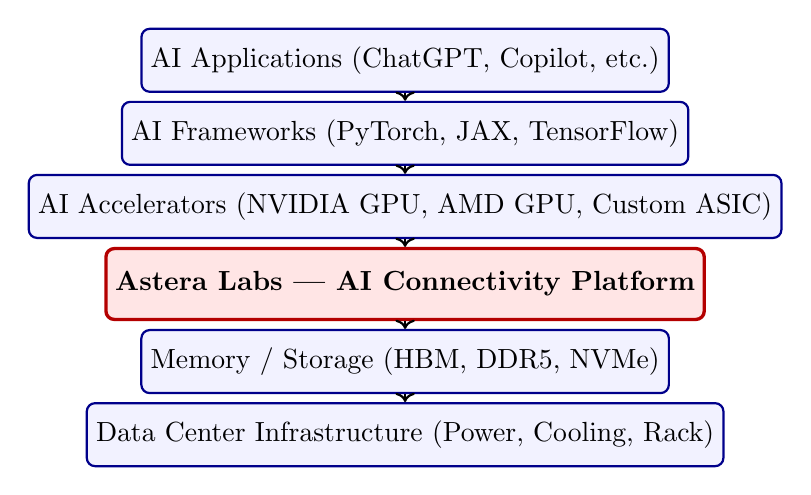
\begin{tikzpicture}[
        node distance=1.4cm,
        layer/.style={rectangle, draw=darkblue, fill=blue!5, thick, minimum width=5cm, minimum height=0.8cm, align=center, rounded corners=3pt},
        highlight/.style={rectangle, draw=darkred, fill=red!10, very thick, minimum width=5cm, minimum height=0.9cm, align=center, rounded corners=3pt}
    ]
        \node[layer] (APP) {AI Applications (ChatGPT, Copilot, etc.)};
        \node[layer, below=0.1cm of APP] (FRAMEWORK) {AI Frameworks (PyTorch, JAX, TensorFlow)};
        \node[layer, below=0.1cm of FRAMEWORK] (GPU) {AI Accelerators (NVIDIA GPU, AMD GPU, Custom ASIC)};
        \node[highlight, below=0.1cm of GPU] (AST) {\textbf{Astera Labs — AI Connectivity Platform}};
        \node[layer, below=0.1cm of AST] (MEM) {Memory / Storage (HBM, DDR5, NVMe)};
        \node[layer, below=0.1cm of MEM] (INFRA) {Data Center Infrastructure (Power, Cooling, Rack)};

        \draw[->, thick] (APP) -- (FRAMEWORK);
        \draw[->, thick] (FRAMEWORK) -- (GPU);
        \draw[->, thick] (GPU) -- (AST);
        \draw[->, thick] (AST) -- (MEM);
        \draw[->, thick] (MEM) -- (INFRA);
    \end{tikzpicture}
    \caption{Astera Labs 在 AI 基础设施堆栈中的位置}
    \label{fig:stack}
\end{figure}

\subsection{投资人视角的三种 Scenario}

\begin{itemize}
    \item \textbf{Bull Case}：Scorpio 成为 AI GPU scale-up 的开放标准，PCIe-based fabric 被所有非 NVIDIA GPU 采用。LTM 收入 3-5 年内达到 \$5B+, 70\%+ 毛利，软件贡献 recurring revenue
    \item \textbf{Base Case}：Scorpio 获得 20-30\% of AI GPU scale-up TAM，Aries 维持 retimer 市场领先地位。收入稳步增长但竞争加剧，毛利率从 75\% 缓慢下降到 65-70\%
    \item \textbf{Bear Case}：Broadcom 快速推出竞争力产品，NVIDIA 扩展 NVLink，CXL adoption 持续缓慢。Astera 的增长大幅放缓，毛利率承压，估值压缩
\end{itemize}

\subsection{最终判断}

\begin{enumerate}
    \item Astera Labs 有\textbf{真实的技术}和\textbf{正确的战略}。SerDes 能力、全栈产品线和 hyperscaler 客户关系构成了真实的价值
    \item 在半导体行业中，``先发优势''的保护期通常在\textbf{2-3 年}。Astera 的价值取决于能否在``窗口期''内建立足够深的客户关系和生态锁定
    \item COSMOS 软件平台是实现长期护城河的\textbf{关键变量}——但它需要在未来 2-3 年内证明自己的锁定效应
    \item 公司最大的 Paradox：NVIDIA GPU 的销售增长直接推动 Astera 的短期收入（更多 GPU 需要更多连接），但 NVIDIA 越封闭（NVLink）Astera 的长期战略价值越高（hyperscaler 更需要开放替代方案）
    \item \textbf{总体评级（非投资建议）}：公司质量 A-, 估值敏感性高（取决于 Scorpio TAM 假设），竞争风险中等偏高
\end{enumerate}


% ============================================================
%  参考文献
% ============================================================
\clearpage
\section{参考文献}
% ============================================================
%  References Appendix
% ============================================================

\phantomsection
\addcontentsline{toc}{subsection}{T1 — 官方可验证文档}
\subsection*{T1 — 官方可验证文档}

\begin{enumerate}[label={[T1-\arabic*]}, leftmargin=*]

    \item \textbf{Astera Labs, Inc. Quarterly and Annual Financial Data (XBRL)}.
    U.S. Securities and Exchange Commission, CIK: 0001736297.
    包含 FY2025 及 Q1 2026 季度/年度营收、毛利、净利。
    \url{https://www.sec.gov/cgi-bin/browse-edgar?CIK=0001736297}

    \item \textbf{Astera Labs, Inc. Form 10-K (FY2025)}, SEC Accession No. 0001736297-26-000010.
    \url{https://www.sec.gov/cgi-bin/viewer?action=view&cik=1736297&accession_number=0001736297-26-000010}

    \item \textbf{PCI Express Base Specification 6.0/6.1}, PCI-SIG.
    \url{https://pcisig.com/}

    \item \textbf{Compute Express Link Specification 1.0 — 4.0}, CXL Consortium.
    \url{https://www.computeexpresslink.org/}

\end{enumerate}

\phantomsection
\addcontentsline{toc}{subsection}{T2 — 官方声明与产品资料}
\subsection*{T2 — 官方声明与产品资料}

\begin{enumerate}[label={[T2-\arabic*]}, leftmargin=*, resume]
    \item \textbf{Astera Labs Official Website — Home, Products, Resources, Blog}.
    \url{https://www.asteralabs.com/}

    \item \textbf{Products Page: Scorpio, Aries, Leo, Taurus, COSMOS}.
    \url{https://www.asteralabs.com/products}

    \item \textbf{Scorpio X-Series Smart Fabric Switch Product Page}.
    \url{https://www.asteralabs.com/products/scorpio}

    \item \textbf{Aries PCIe/CXL Smart DSP Retimers \& Interop Reports}.
    \url{https://www.asteralabs.com/products/aries}

    \item \textbf{Leo CXL Smart Memory Controllers \& Interop Reports}.
    \url{https://www.asteralabs.com/products/leo}

    \item \textbf{COSMOS Connectivity System Management and Optimization Software}.
    \url{https://www.asteralabs.com/products/cosmos}

    \item \textbf{Resources: White Papers, Application Notes, Webinars}.
    \url{https://www.asteralabs.com/resources/}

    \item \textbf{White Papers}: ``Reinventing the Backplane'', ``Migrating AI Server Designs to Scorpio'',
    ``Overcome Next-Gen AI Infrastructure Challenges with Scorpio'', ``Cloud Fleet Management with COSMOS''.
    \url{https://www.asteralabs.com/resources/white-papers/}

    \item \textbf{Application Notes}: Leo Product Design Guide, Leo Software, Aries Self Test,
    Aries Security, Aries RX Lane Margining, etc.
    \url{https://www.asteralabs.com/document-requests/}

    \item \textbf{Blog}: Caleb Shetland, ``Why Your Mixture-of-Experts Model Is Only as Good as Your Fabric''.
    \url{https://www.asteralabs.com/blog/why-your-mixture-of-experts-model-is-only-as-good-as-your-fabric}

    \item \textbf{Blog}: Thad Omura, ``Why Connectivity is the New Frontier of AI Infrastructure—and What NVLink Fusion Means for the Future''.
    \url{https://www.asteralabs.com/blog/}

    \item \textbf{Blog}: Amit Golander, PhD, ``Inference Tokenomics: How CXL Memory Expansion Improves AI Economics''.
    \url{https://www.asteralabs.com/blog/}

    \item \textbf{Blog}: Jignesh Shah, ``Enabling Multi-Rack AI Clusters with Aries Smart Cable Modules for PCIe 6''.
    \url{https://www.asteralabs.com/blog/enabling-multi-rack-ai-clusters-with-aries-smart-cable-modules-for-pcie-6}

    \item \textbf{Blog}: Abhishek Wadhwa, ``Bridge the PCIe 6 Transition Without Requalifying Your NIC Fleet''.
    \url{https://www.asteralabs.com/blog/}

    \item \textbf{Investor Relations — Q1 2026 Earnings Release}.
    \url{https://ir.asteralabs.com/}

    \item \textbf{Arm Total Design Ecosystem (Astera Labs Joins)}, Press Release (Late 2025).

    \item \textbf{Wikipedia}, ``Astera Labs''.
    \url{https://en.wikipedia.org/wiki/Astera_Labs}
    (Note: has notability/COI flags as of Feb 2026)

\end{enumerate}

\phantomsection
\addcontentsline{toc}{subsection}{T3 — 第三方权威分析}
\subsection*{T3 — 第三方权威分析}

\begin{enumerate}[label={[T3-\arabic*]}, leftmargin=*, resume]
    \item \textbf{SemiAnalysis (Dylan Patel et al.)}, ``Astera Labs IPO: The Next Connectivity Giant?'',
    March 17, 2024.
    \url{https://newsletter.semianalysis.com/p/astera-labs-ipo-the-next-connectivity}

    \item \textbf{Wikipedia}, ``Compute Express Link''.
    \url{https://en.wikipedia.org/wiki/Compute_Express_Link}

    \item \textbf{Wikipedia}, ``Memory Wall''.
    \url{https://en.wikipedia.org/wiki/Memory_wall}
\end{enumerate}

\phantomsection
\addcontentsline{toc}{subsection}{T4 — 行业媒体与分析}
\subsection*{T4 — 行业媒体与分析}

\begin{enumerate}[label={[T4-\arabic*]}, leftmargin=*, resume]
    \item \textbf{CXL Consortium Blog}, ``CXL 4.0 Specification Webinar Q\&A'', etc.
    \url{https://www.computeexpresslink.org/blog}

    \item \textbf{ServeTheHome} (attempted, blocked by permission/Cloudflare restrictions during research).
    \url{https://www.servethehome.com/}

    \item \textbf{AnandTech} (attempted, blocked by permission restrictions during research).
    \url{https://www.anandtech.com/}
\end{enumerate}

\phantomsection
\addcontentsline{toc}{subsection}{竞品参考来源}
\subsection*{竞品参考来源}

\begin{enumerate}[label={[COMP-\arabic*]}, leftmargin=*, resume]
    \item \textbf{Credo Technology}, Product Portfolio (Dove Retimers, HiWire AECs).
    \url{https://www.credo-technology.com/products}

    \item \textbf{Broadcom Inc.}, PEX Series PCIe Switches and Retimers.
    \url{https://www.broadcom.com/products/pcie-switches-retimers}

    \item \textbf{Microchip Technology}, Switchtec PCIe Switch Family.
    \url{https://www.microchip.com/}

    \item \textbf{Open Compute Project (OCP)}, Global Summit Presentations \& Specifications.
    \url{https://www.opencompute.org/}
\end{enumerate}

\phantomsection
\addcontentsline{toc}{subsection}{未验证/待补充来源}
\subsection*{待补充的研究来源}

以下来源在研究计划中被识别但未能在本次调研中充分访问（受权限、paywall 或 API 限制）：

\begin{itemize}
    \item USPTO / Google Patents —— Astera Labs 专利组合检索
    \item Gartner / IDC —— AI Connectivity TAM 详细报告 (paywalled)
    \item Hot Chips / ISSCC —— Astera Labs conference proceedings
    \item OCP Summit —— Astera Labs specific presentations (需 OCP portal 权限)
    \item Astera Labs YouTube Channel —— Product demos and technical talks
    \item Third-party benchmark data (如 AnandTech/ServeTheHome 的实测)
\end{itemize}


% ============================================================
%  附录：研究方法与限制
% ============================================================
\clearpage
\section*{附录A：研究方法论与限制}
\addcontentsline{toc}{section}{附录A：研究方法论与限制}

\textbf{信息来源总结}：
\begin{itemize}
    \item \textbf{T1 (官方可验证)}：SEC XBRL 财报数据、PCIe/CXL 公开规范
    \item \textbf{T2 (官方声明)}：官网产品页、官方博客、interop reports、白皮书
    \item \textbf{T3 (第三方权威)}：SemiAnalysis IPO 分析、Wikipedia (CXL, Memory Wall)
    \item \textbf{T4 (行业媒体)}：曾尝试访问 ServeTheHome/AnandTech/The Next Platform（部分受 Cloudflare/权限限制）
    \item \textbf{T5 (推测/未确认)}：所有标注 \unverified{} 和 \speculation{} 的内容
\end{itemize}

\textbf{已知信息缺口}：
\begin{enumerate}
    \item Scorpio 端到端延迟、功耗、die size —— 未公开
    \item 精确客户名单和收入占比 —— 未公开（集中度风险仅能从 SemiAnalysis 推断）
    \item 各产品线的收入拆分 —— 未公开
    \item 专利数量和质量 —— 未检索
    \item 与 NVIDIA 的正式合作关系细节 —— NVLink Fusion 博客未完全公开
    \item 各代产品的 ASP（平均售价）—— 未公开
    \item OCP/CXL Consortium 中 Astera Labs 的具体贡献细节 —— 需要访问 OCP portal
\end{enumerate}

\textbf{后续研究建议}：
\begin{itemize}
    \item 专利检索：USPTO / Google Patents 检索 "Astera Labs" 专利组合
    \item Conference 分析：Hot Chips / ISSCC / OCP Summit 中 Astera Labs 的演讲
    \item 竞品对比：Broadcom PEX 系列、Credo Dove 系列的实际性能对比
    \item 供应链验证：TSMC 具体制程节点、封测厂确认
\end{itemize}

\end{document}
